
%\section*{Appendix: Extra Experiments}
%\label{sec:appendix}

%\subsection{Case Study for Feature Extraction}

\begin{figure*}
  \centering
  \subfigure[]{
  \label{fig:subfig1:fig11}
      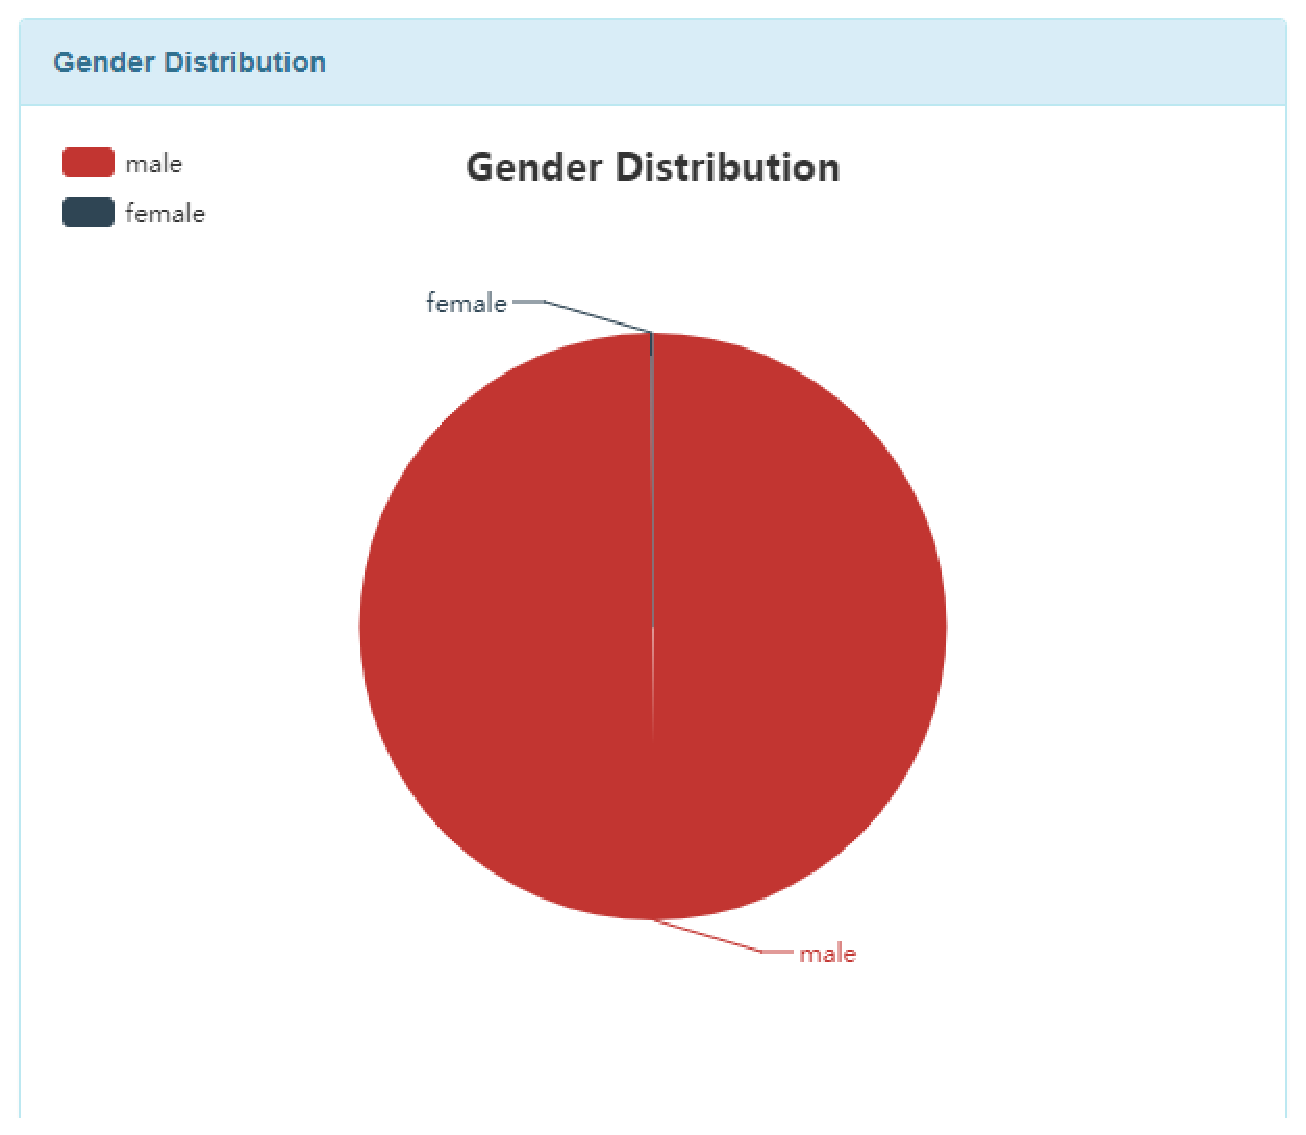
\includegraphics[width=0.23\textwidth]{IMAGE/group-images/11.eps}}
  \subfigure[]{
  \label{fig:subfig1:fig12}
      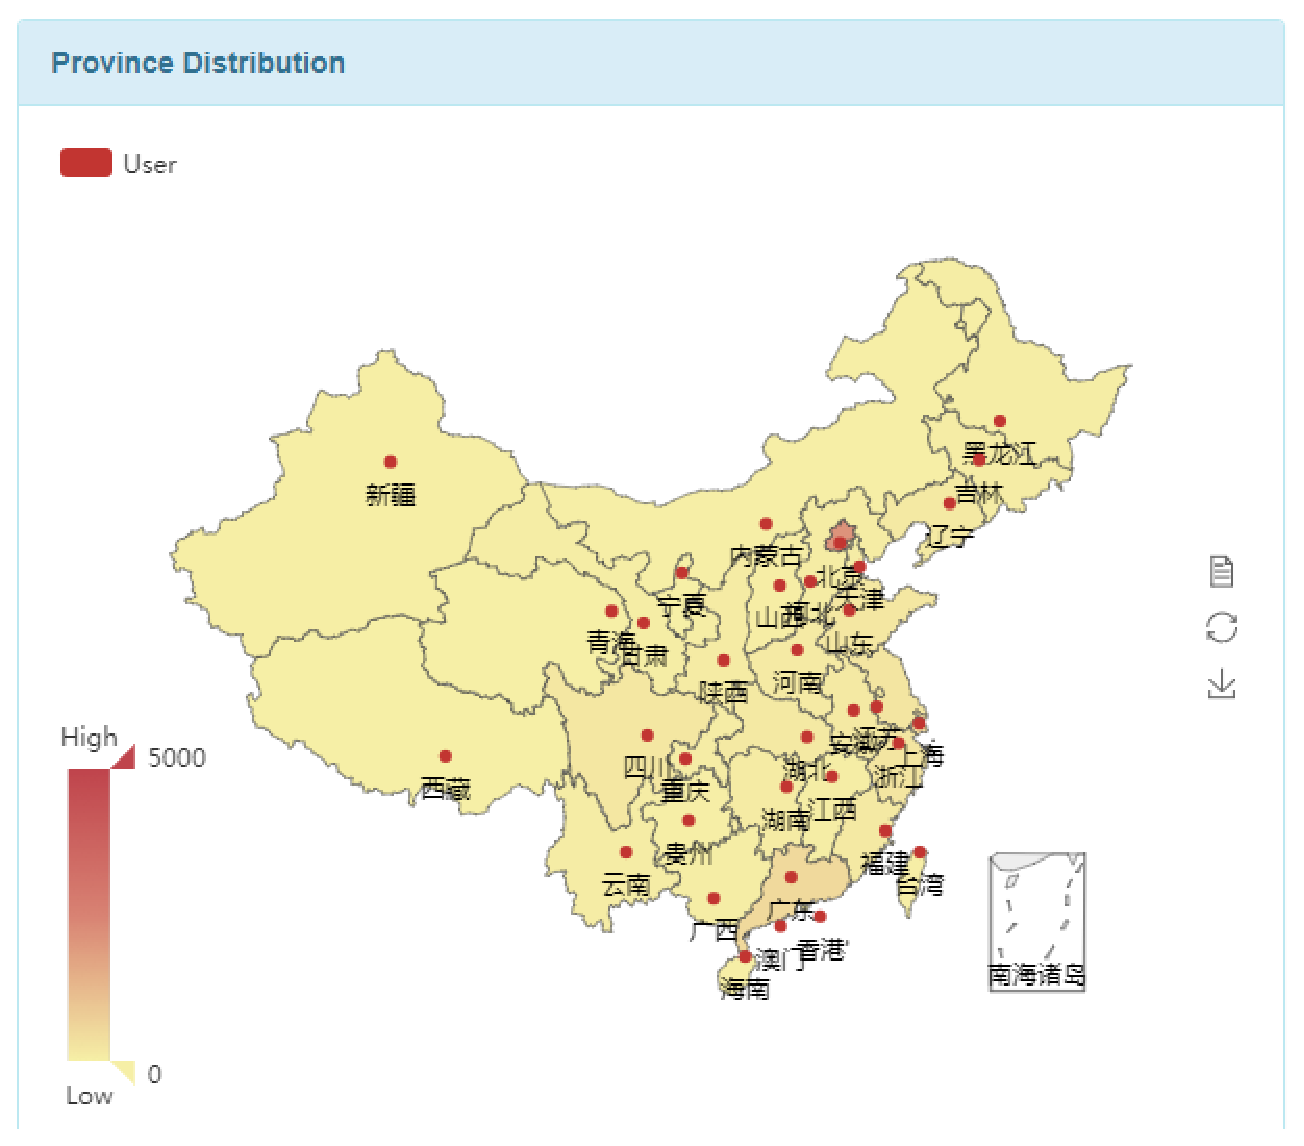
\includegraphics[width=0.23\textwidth]{IMAGE/group-images/12.eps}}
  \subfigure[]{
  \label{fig:subfig1:fig13}
      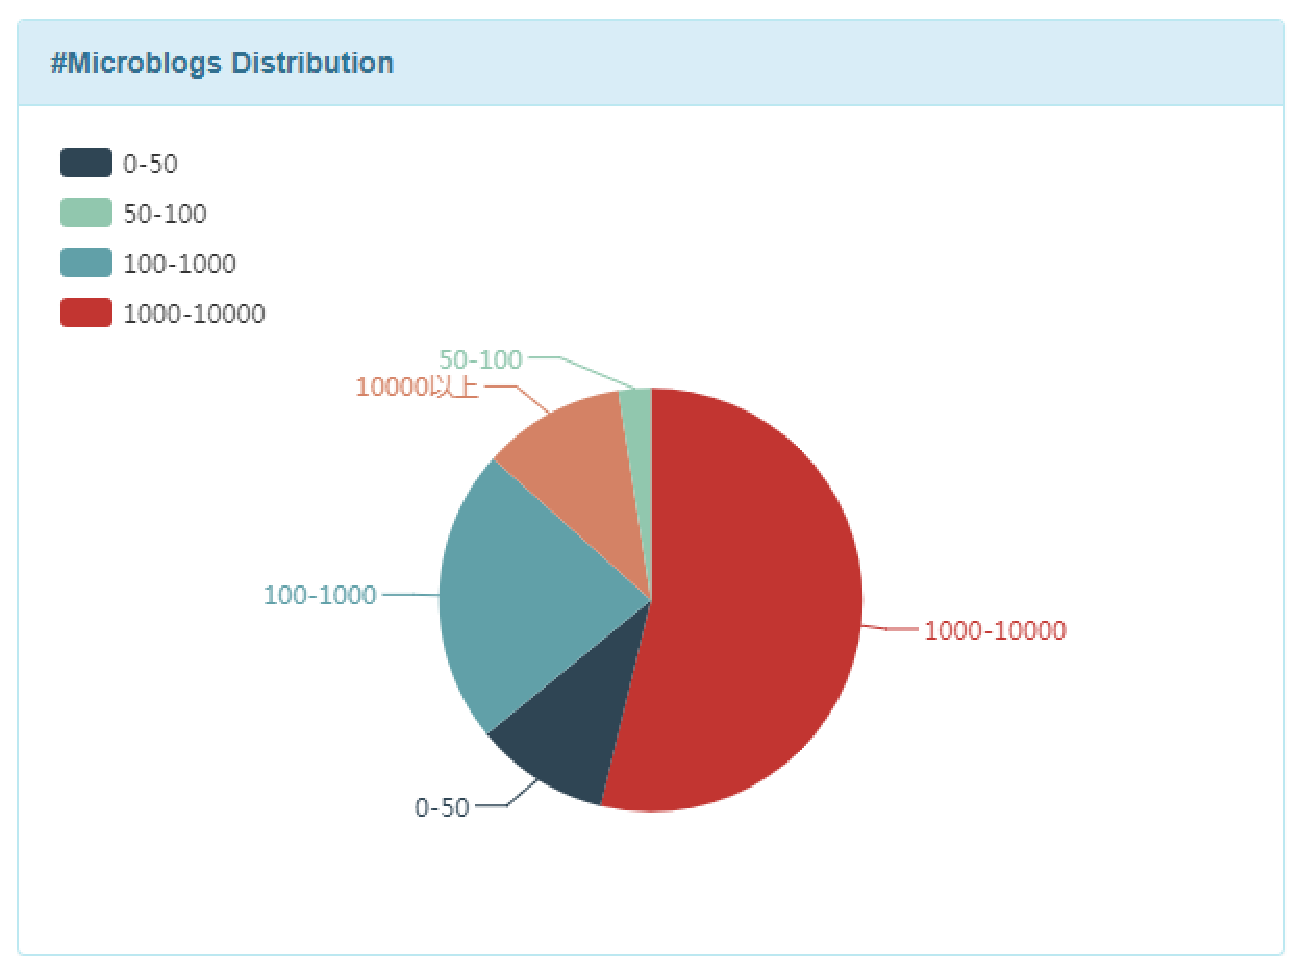
\includegraphics[width=0.23\textwidth]{IMAGE/group-images/13.eps}}
  \subfigure[]{
  \label{fig:subfig1:fig14}
      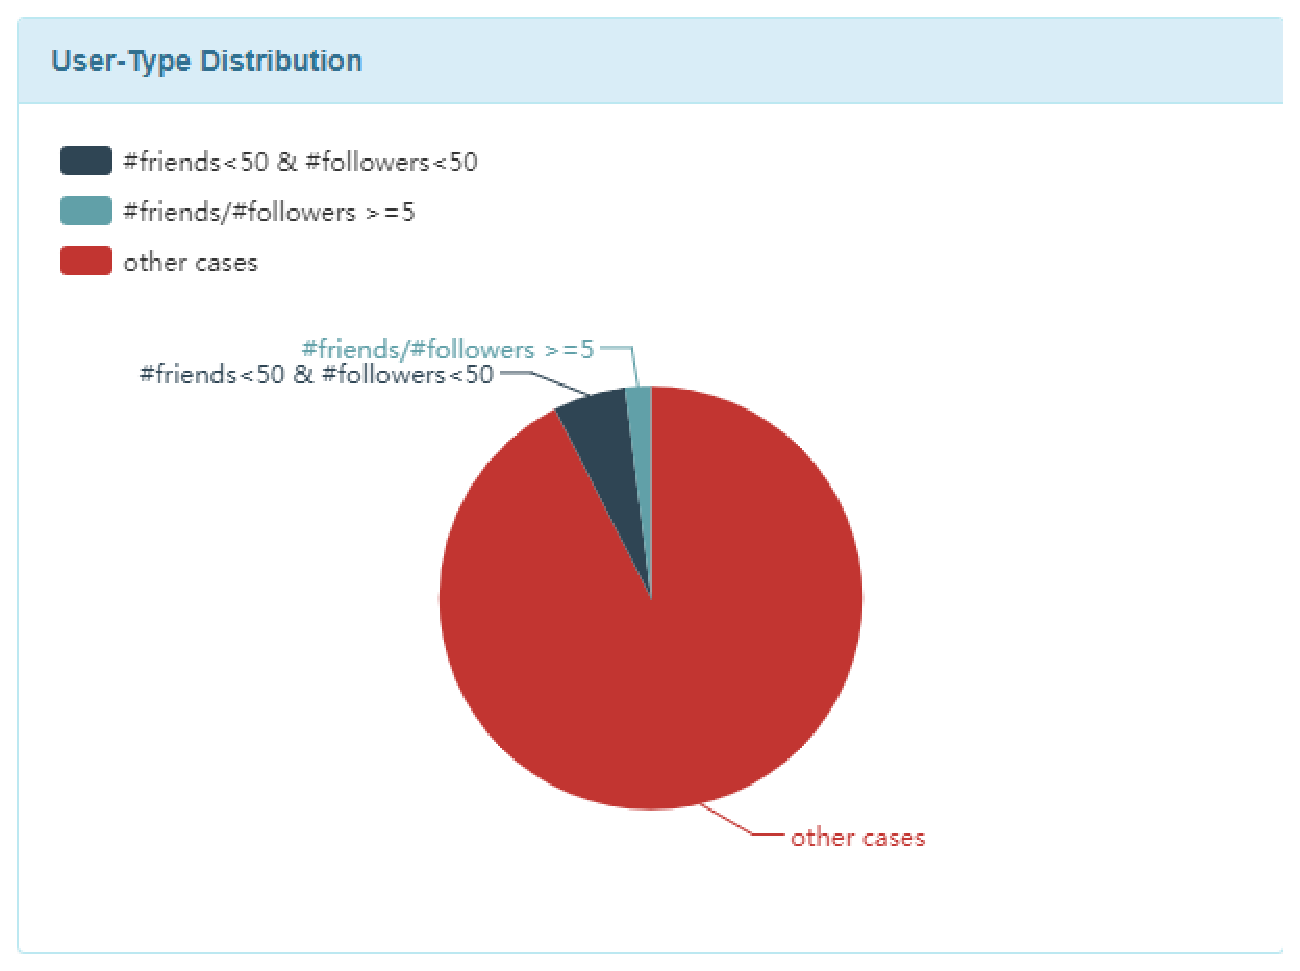
\includegraphics[width=0.23\textwidth]{IMAGE/group-images/14.eps}}
  \subfigure[]{
  \label{fig:subfig1:fig15}
      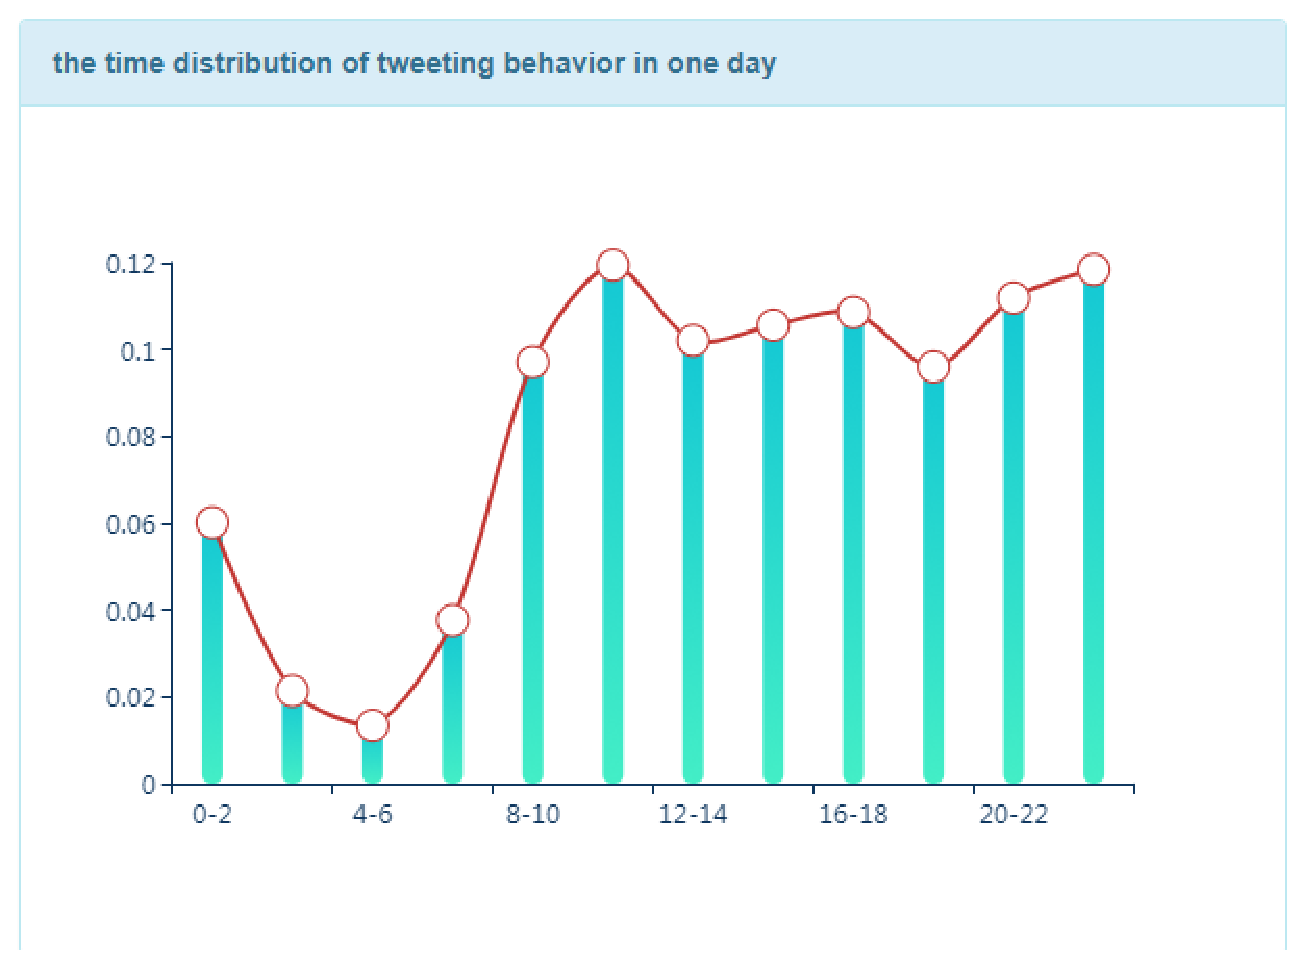
\includegraphics[width=0.23\textwidth]{IMAGE/group-images/15.eps}}
  \subfigure[]{
  \label{fig:subfig1:fig16}
      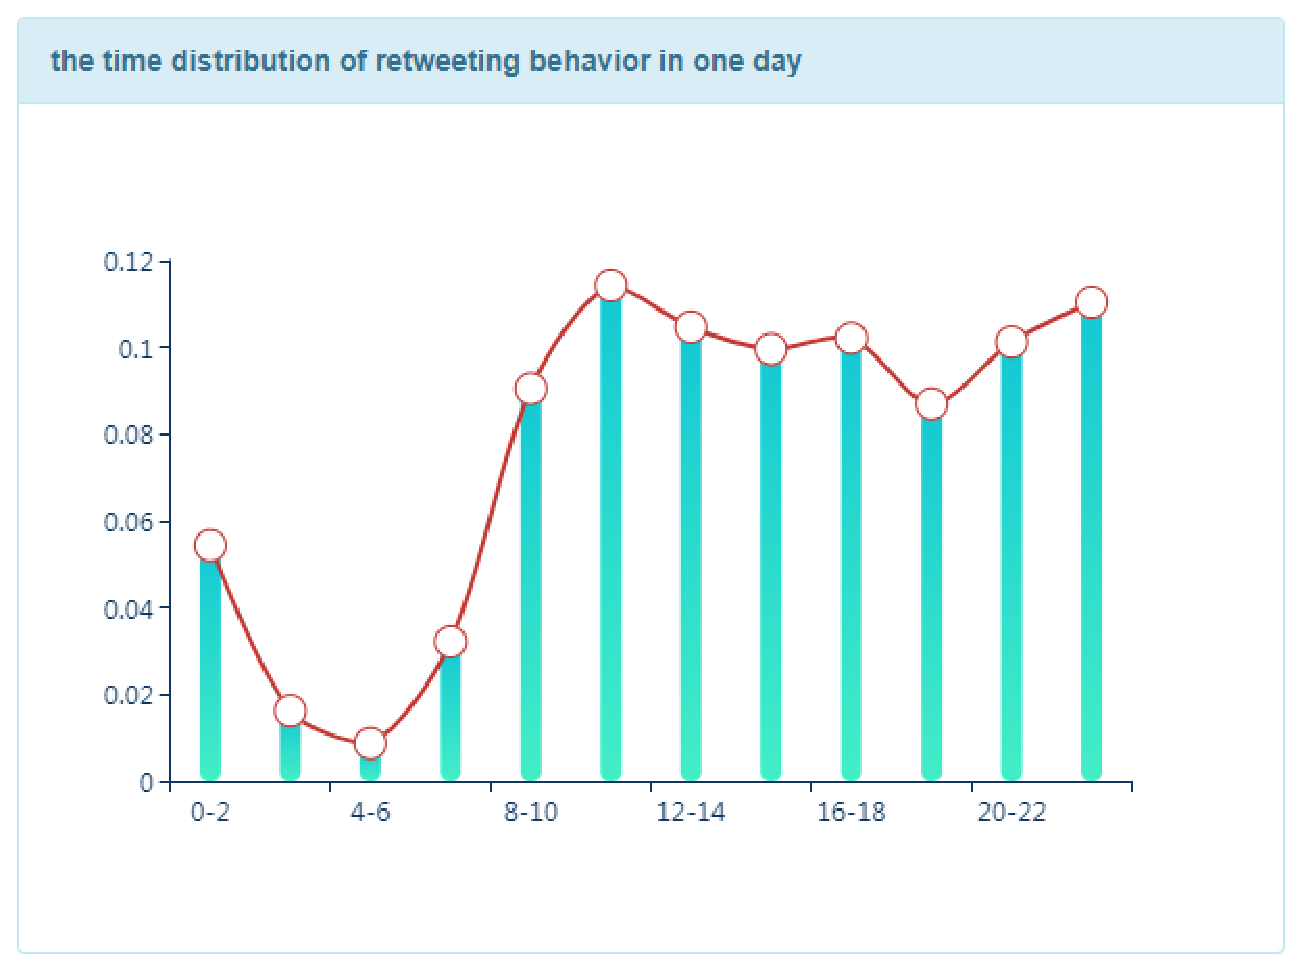
\includegraphics[width=0.23\textwidth]{IMAGE/group-images/16.eps}}
  \subfigure[]{
  \label{fig:subfig1:fig17}
      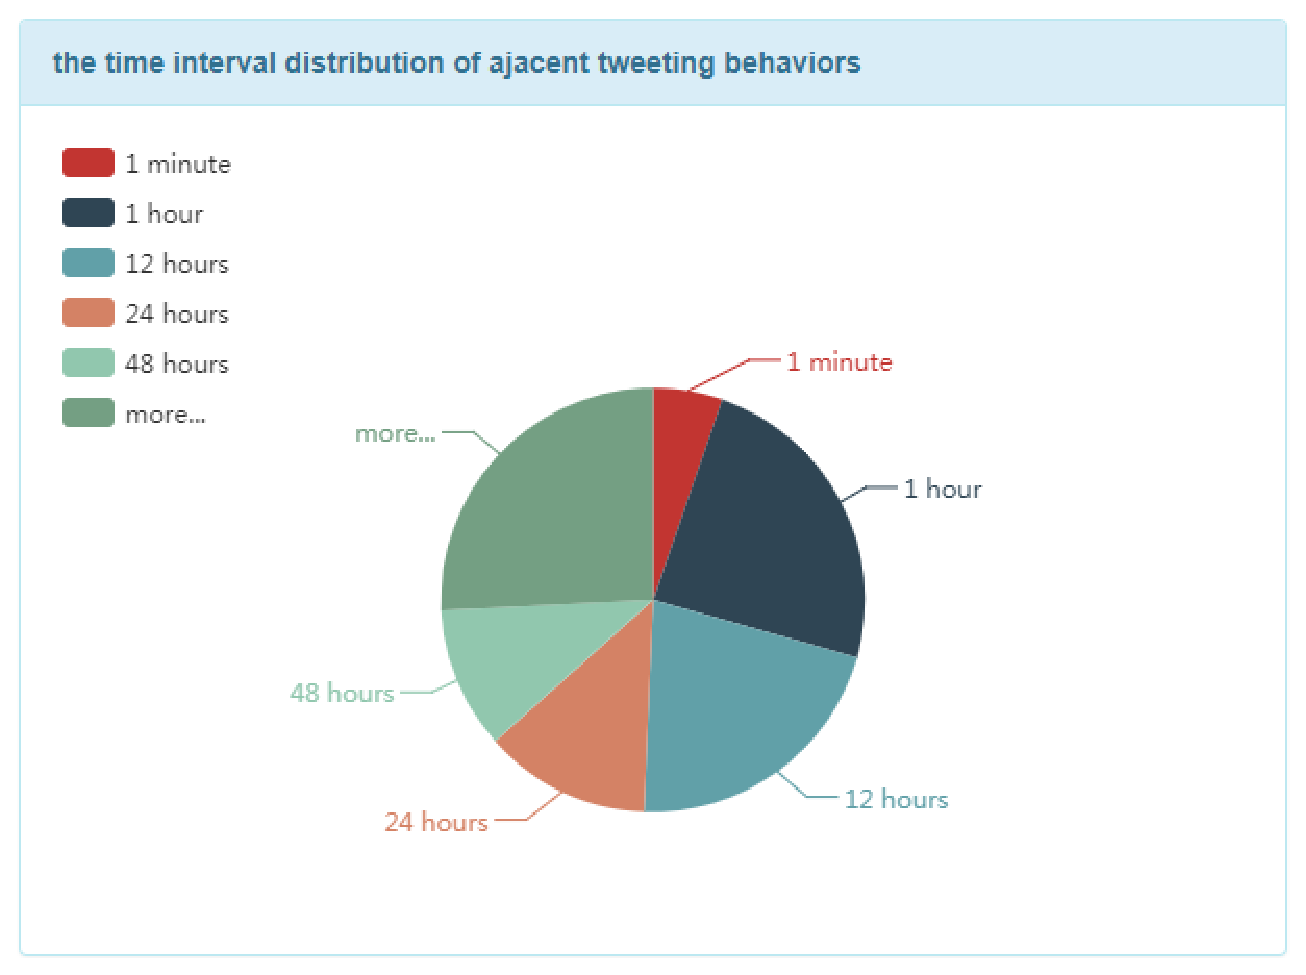
\includegraphics[width=0.23\textwidth]{IMAGE/group-images/17.eps}}
  \subfigure[]{
  \label{fig:subfig1:fig18}
      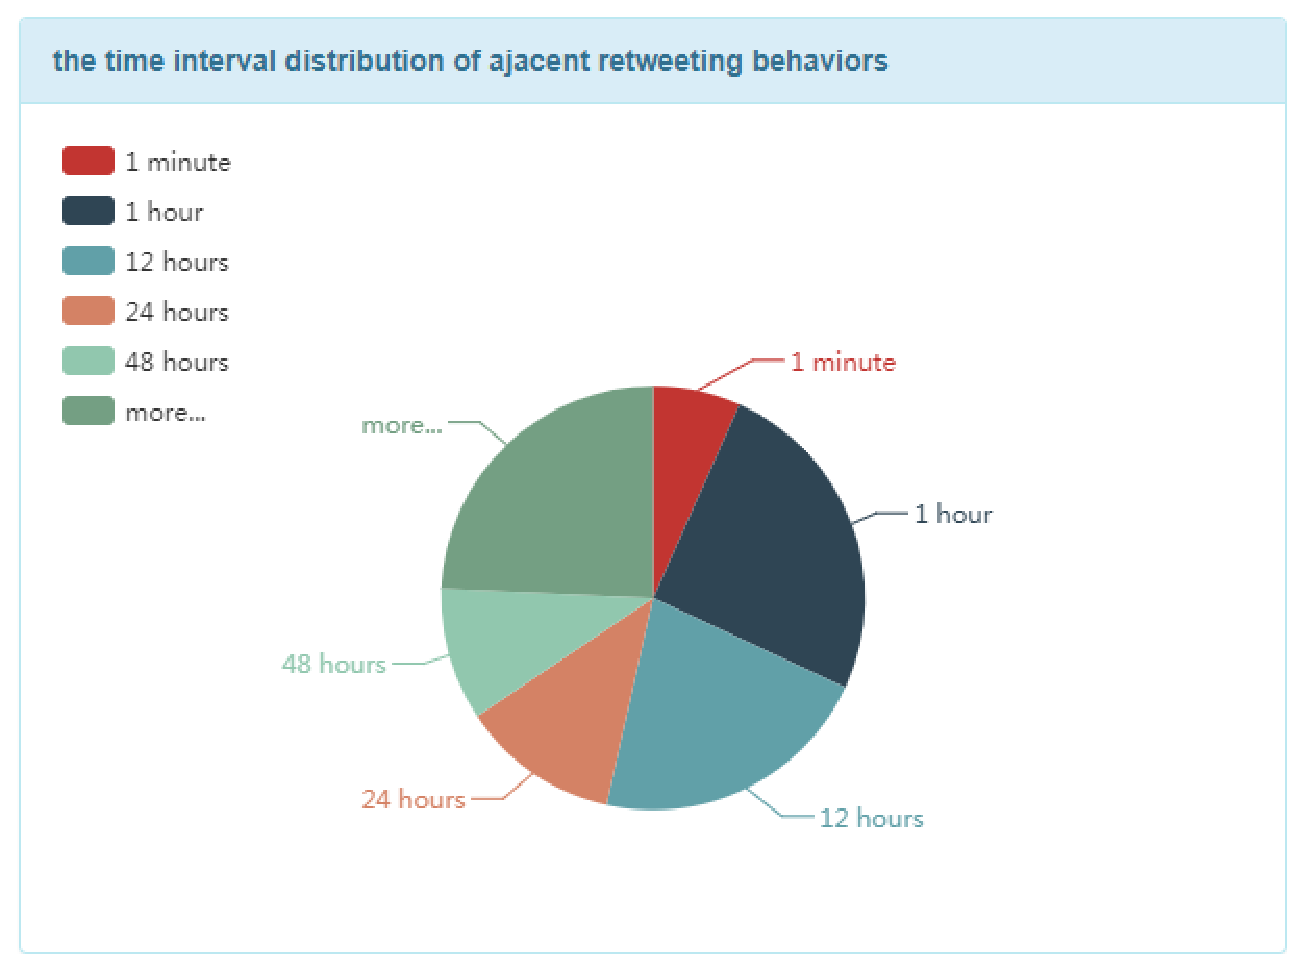
\includegraphics[width=0.23\textwidth]{IMAGE/group-images/18.eps}}
  \subfigure[]{
  \label{fig:subfig1:fig19}
      
\includegraphics[width=0.23\textwidth]{IMAGE/group-images/19.eps}}
  \caption{The Statistics of User Group One}
  \label{fig:subfig1} %% label for entire figure
\end{figure*}
\subsection*{Exp-5: Case Study for User Clustering}

In this section, we show the results of \sys{} for User Clustering. We carefully analyzed the statistical information of four groups obtained from user clustering.

\stab(1) Most users of group one are male (as shown in Fig. \ref{fig:subfig1:fig11}), and Fig. \ref{fig:subfig1:fig12} shows that they are mainly in Beijing(����). The amount of their followees is mostly similar as their followers (as shown in Fig. \ref{fig:subfig1:fig14}). The most active time of this group is mainly between 10 am and 12 am (as shown in Fig. \ref{fig:subfig1:fig15} and \ref{fig:subfig1:fig16}).

\stab(2) Mostly users of group two are  female (as shown in Fig. \ref{fig:subfig2:fig21}) and are also mainly in Beijing (����) (shown as Fig. \ref{fig:subfig2:fig22}). Similar to group one, most of them have followees close to followers (as shown in Fig. \ref{fig:subfig2:fig24}). The most active time of this group is mainly between 10 pm and 12 pm (as shown in Fig. \ref{fig:subfig2:fig25} and \ref{fig:subfig2:fig26}).

\stab(3) Most users of group three are male (as shown in Fig. \ref{fig:subfig3:fig31}). They come from a wide range of provinces (as shown in Fig. \ref{fig:subfig3:fig32}). Most of them have number of followers far more than followees (as shown in Fig. \ref{fig:subfig3:fig34}). The most active time of this group is mainly in 10-12 am and 10-12 pm (as shown in Fig. \ref{fig:subfig3:fig35} and \ref{fig:subfig3:fig36}).

\stab(4) Most users of group four are female (as shown in Fig. \ref{fig:subfig4:fig41}), and they come from a wide range of provinces just as group three (as shown in Fig. \ref{fig:subfig4:fig42}). Most of these users have the amount  of followers far more than followees (as shown in Fig. \ref{fig:subfig4:fig44}). And the most active time of these users is mainly between 10 pm and 12 pm (as shown in Fig. \ref{fig:subfig4:fig45} and \ref{fig:subfig4:fig46}).

According to Fig. \ref{fig:subfig1:fig13}, \ref{fig:subfig2:fig23}, \ref{fig:subfig3:fig33} and \ref{fig:subfig4:fig43},
the number distribution of microblogs for four groups is similar with each other.
We visualize each group's long-term interest expressed as words cloud (shown in Figs. \ref{fig:subfig1:fig19}, \ref{fig:subfig2:fig29}, \ref{fig:subfig3:fig39} and \ref{fig:subfig4:fig49}). As we can see, group one and group three have similar interests.


\begin{figure*}
  \centering
  \subfigure[]{
  \label{fig:subfig2:fig21}
      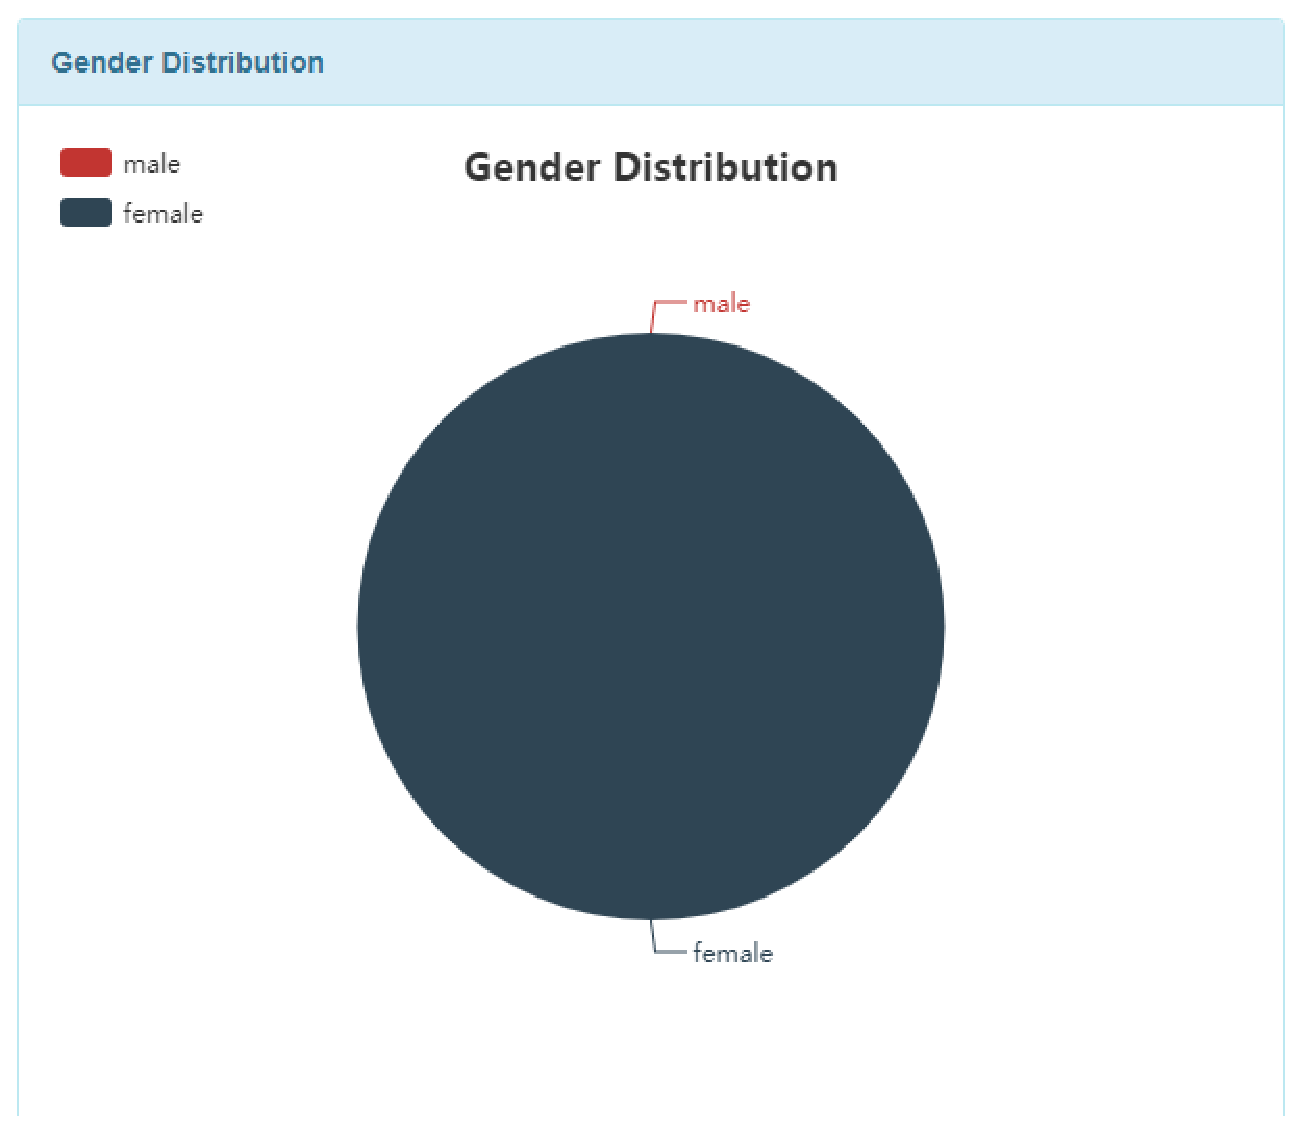
\includegraphics[width=0.23\textwidth]{IMAGE/group-images/21.eps}}
  \subfigure[]{
  \label{fig:subfig2:fig22}
      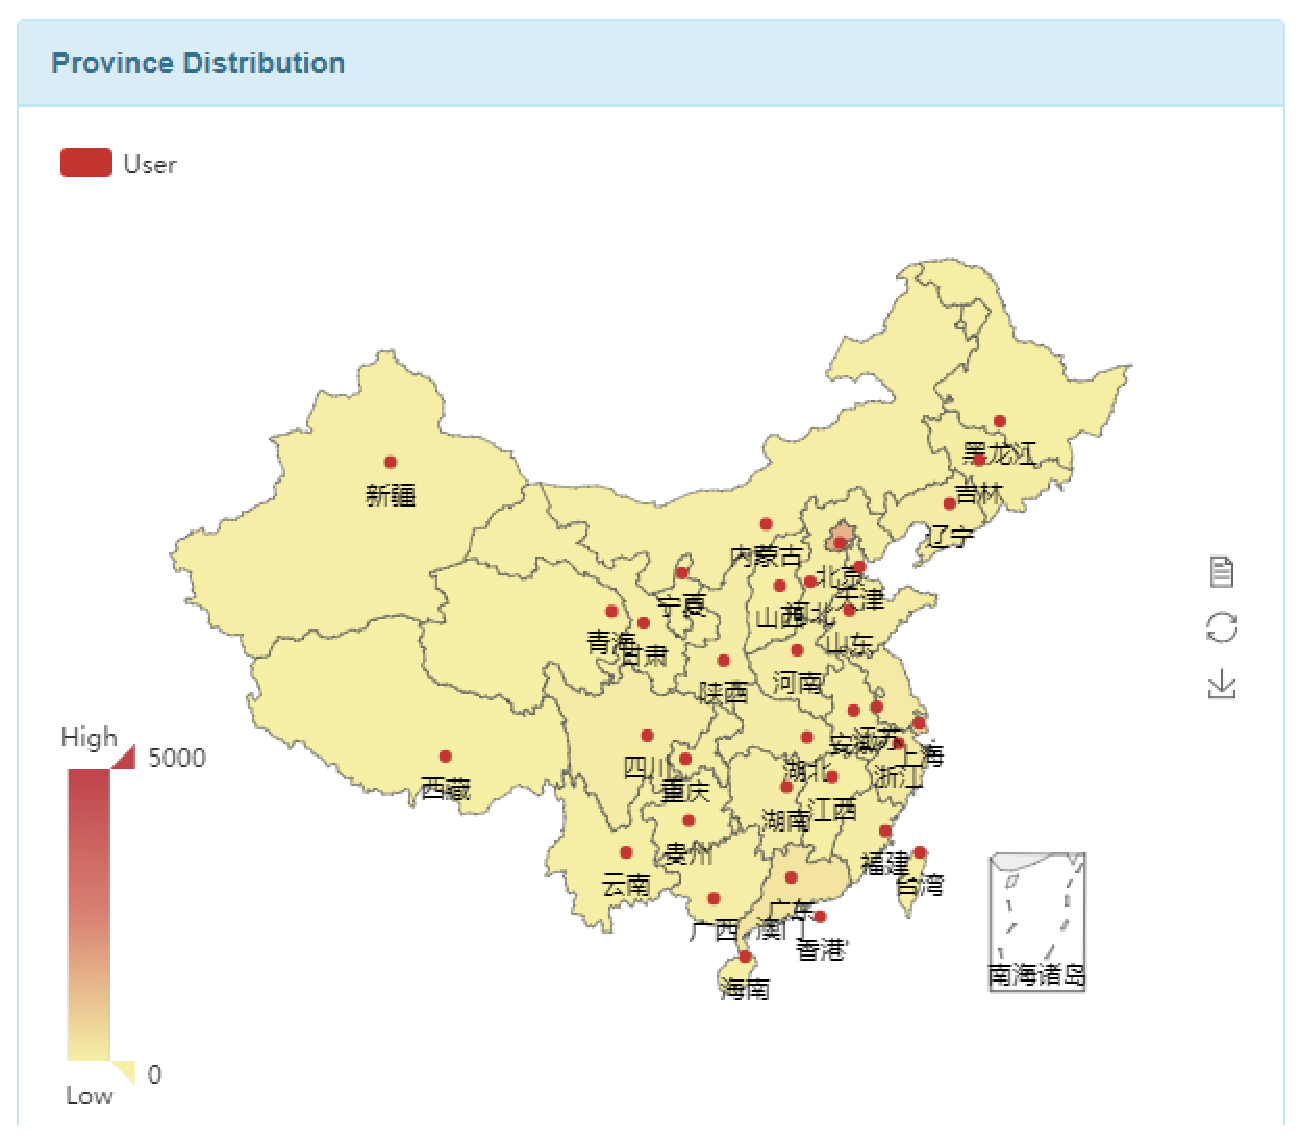
\includegraphics[width=0.23\textwidth]{IMAGE/group-images/22.eps}}
  \subfigure[]{
  \label{fig:subfig2:fig23}
      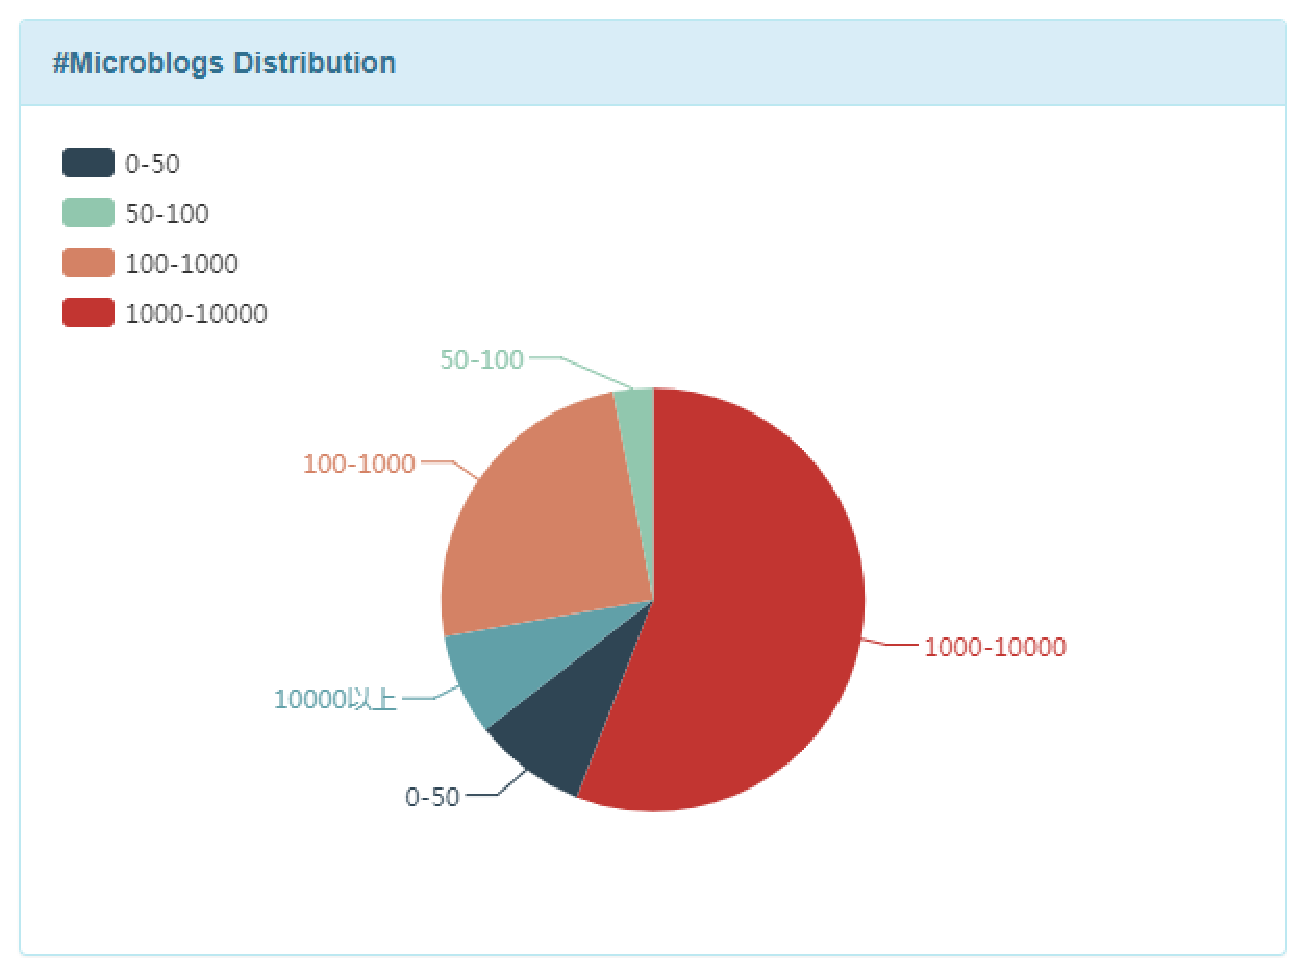
\includegraphics[width=0.23\textwidth]{IMAGE/group-images/23.eps}}
  \subfigure[]{
  \label{fig:subfig2:fig24}
      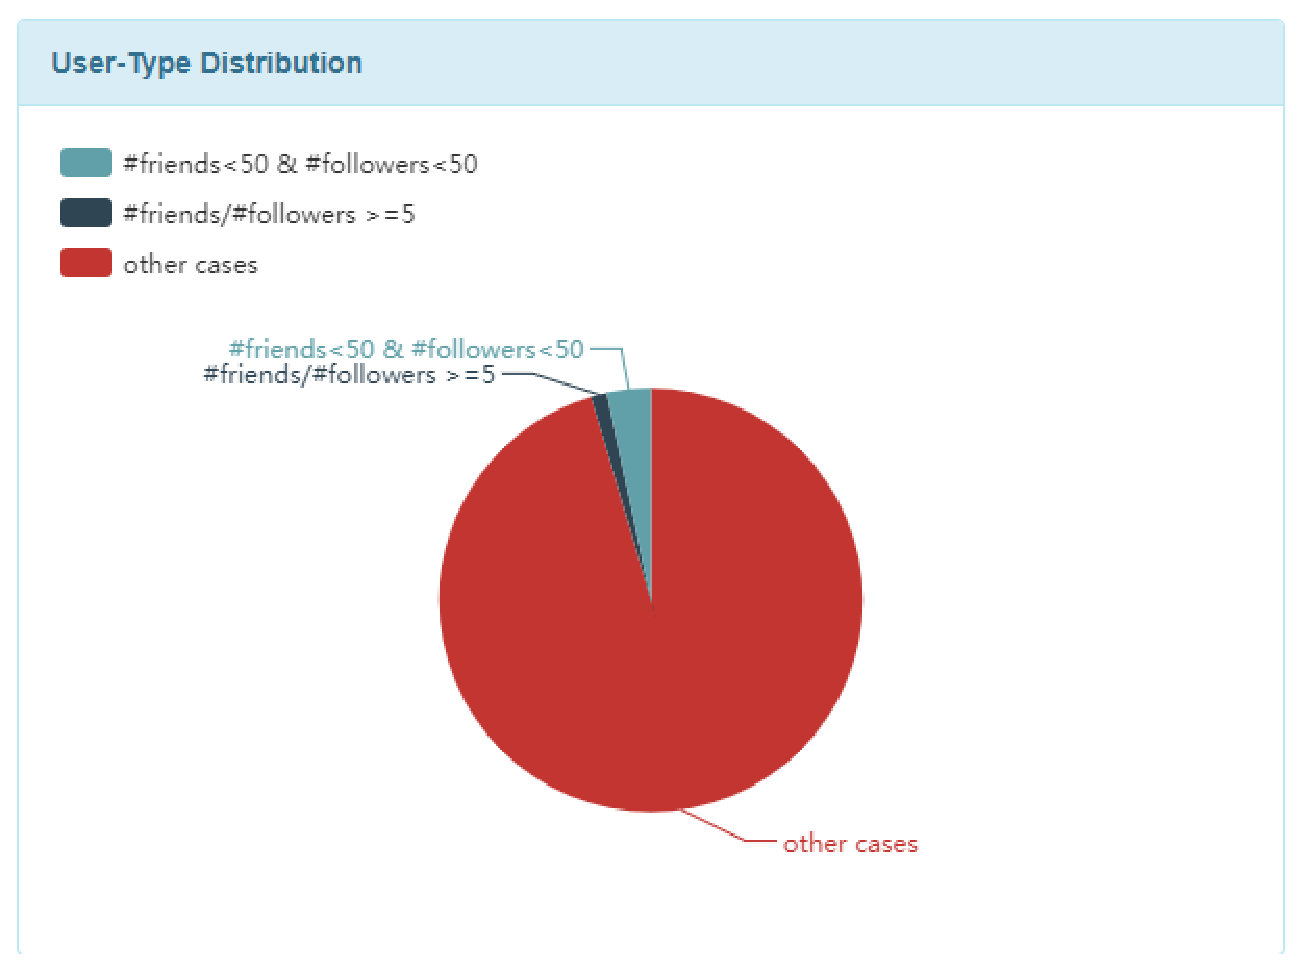
\includegraphics[width=0.23\textwidth]{IMAGE/group-images/24.eps}}
  \subfigure[]{
  \label{fig:subfig2:fig25}
      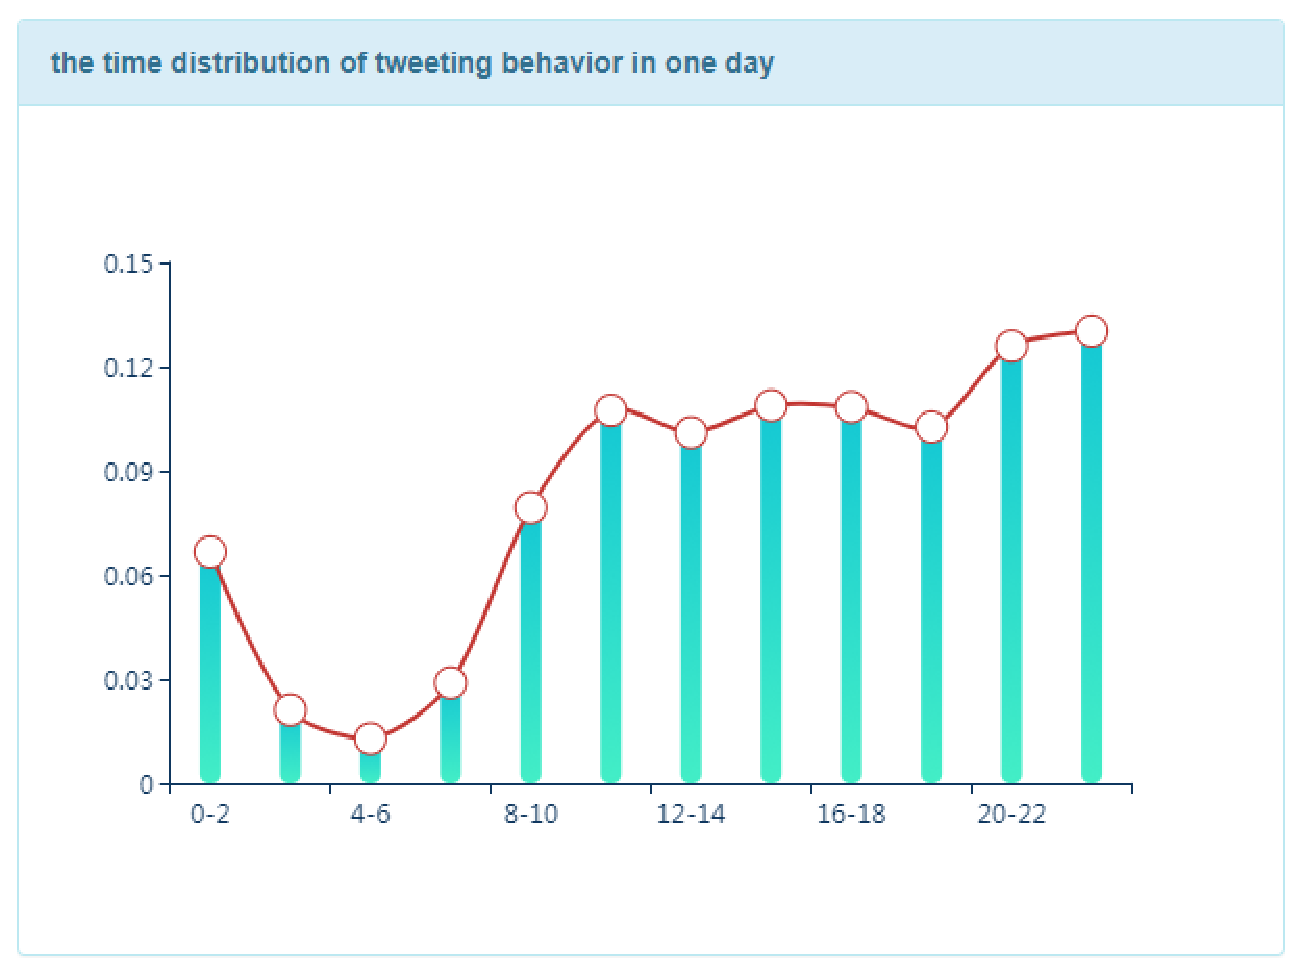
\includegraphics[width=0.23\textwidth]{IMAGE/group-images/25.eps}}
  \subfigure[]{
  \label{fig:subfig2:fig26}
      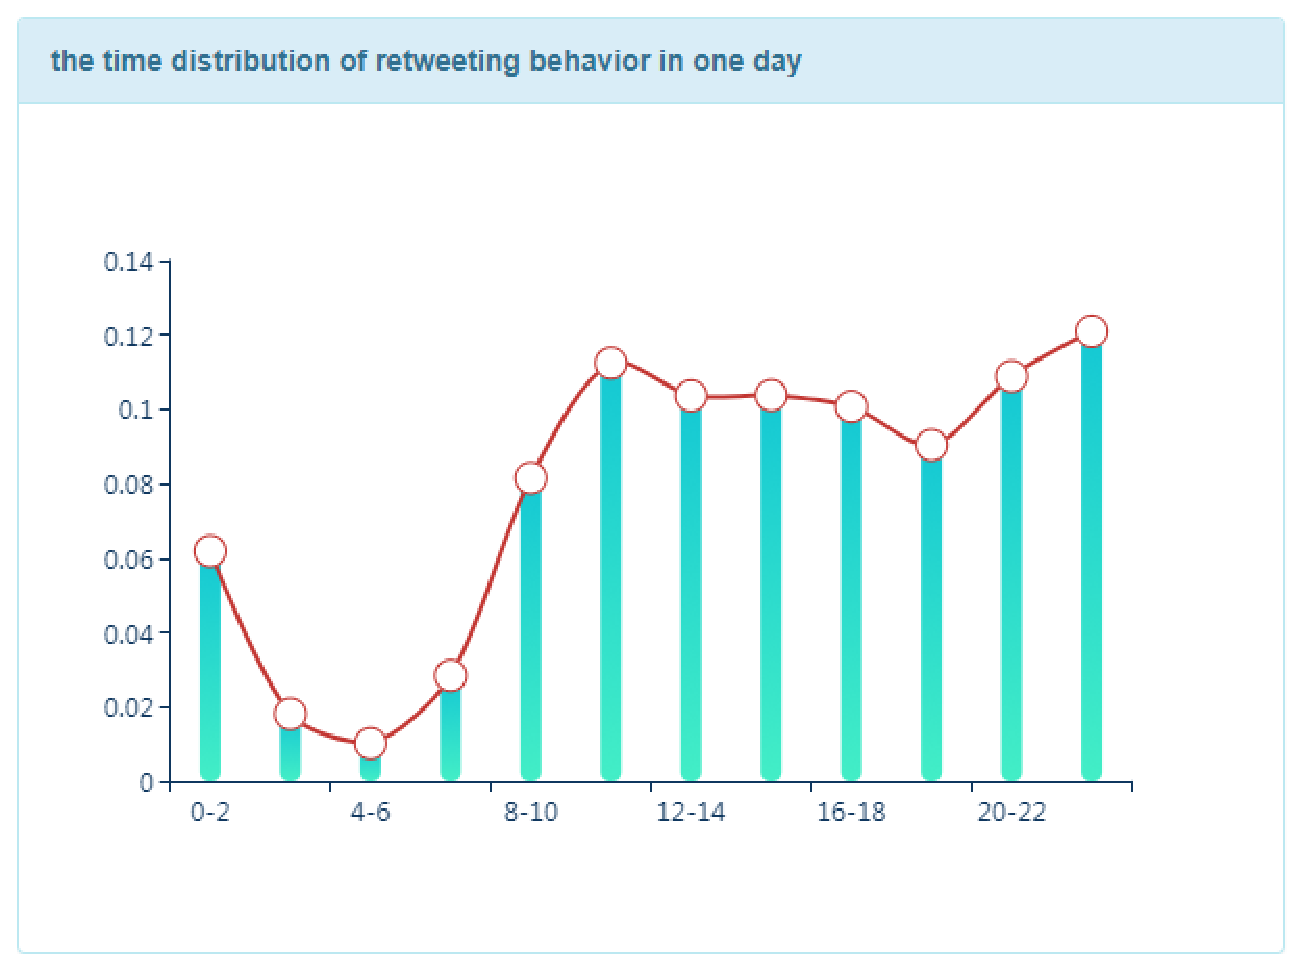
\includegraphics[width=0.23\textwidth]{IMAGE/group-images/26.eps}}
  \subfigure[]{
  \label{fig:subfig2:fig27}
      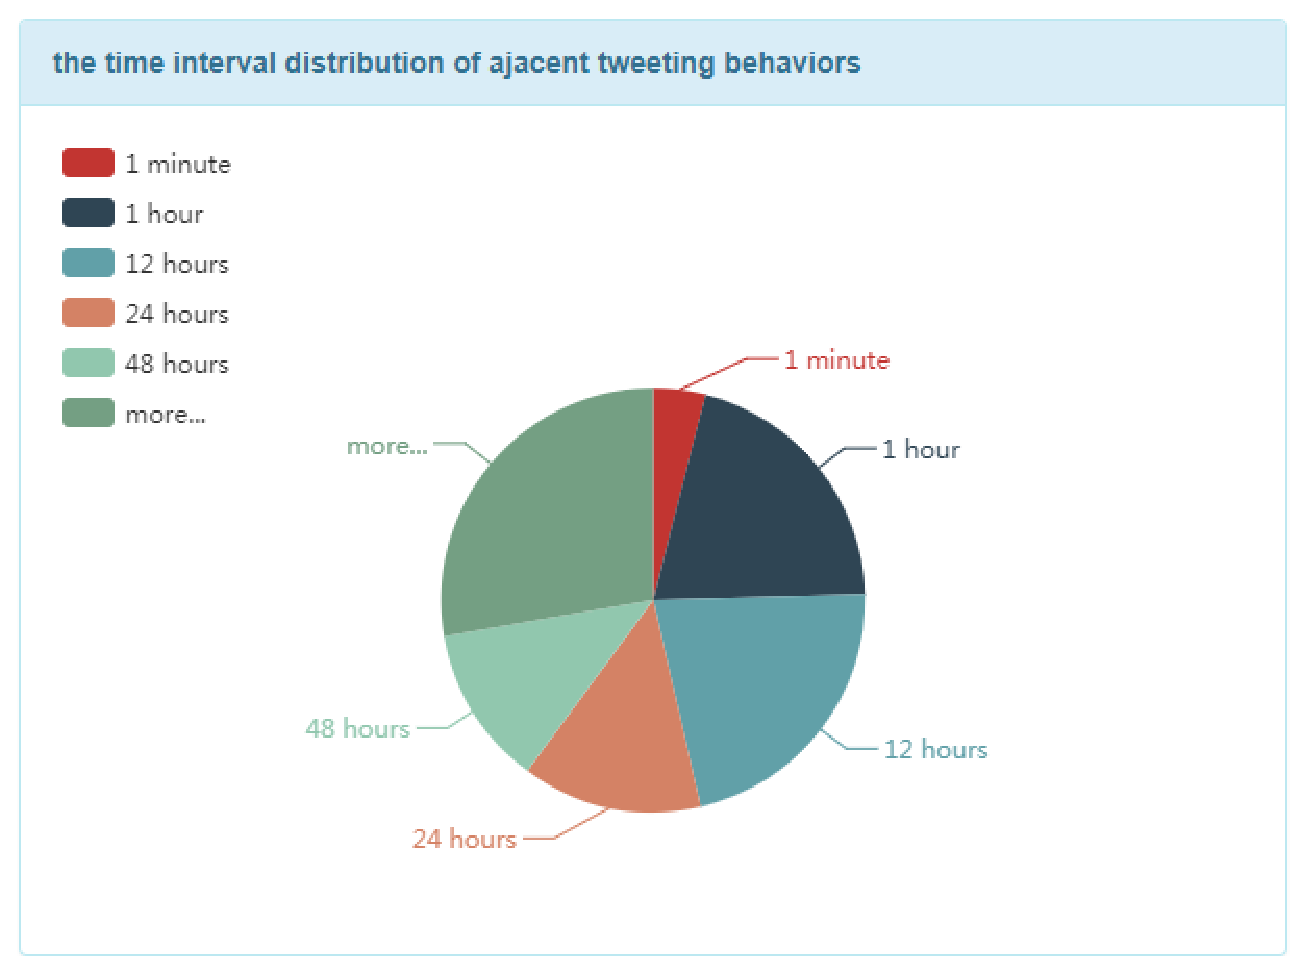
\includegraphics[width=0.23\textwidth]{IMAGE/group-images/27.eps}}
  \subfigure[]{
  \label{fig:subfig2:fig28}
      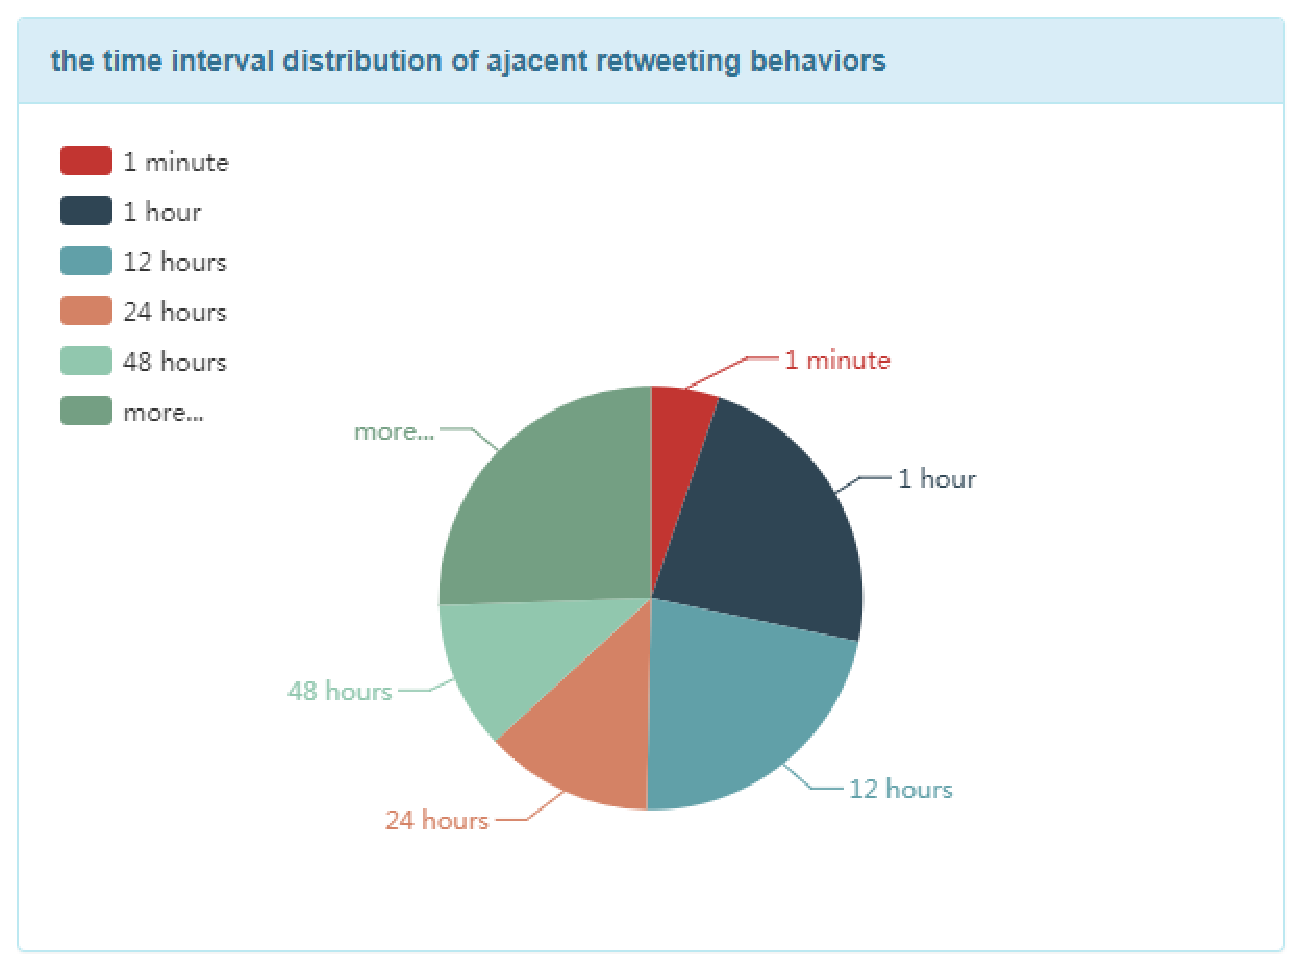
\includegraphics[width=0.23\textwidth]{IMAGE/group-images/28.eps}}
  \subfigure[]{
  \label{fig:subfig2:fig29}
      
\includegraphics[width=0.23\textwidth]{IMAGE/group-images/29.eps}}
  \caption{The Statistics of User Group Two}
  \label{fig:subfig2} %% label for entire figure
\end{figure*}

\begin{figure*}
  \centering
  \subfigure[]{
  \label{fig:subfig3:fig31}
      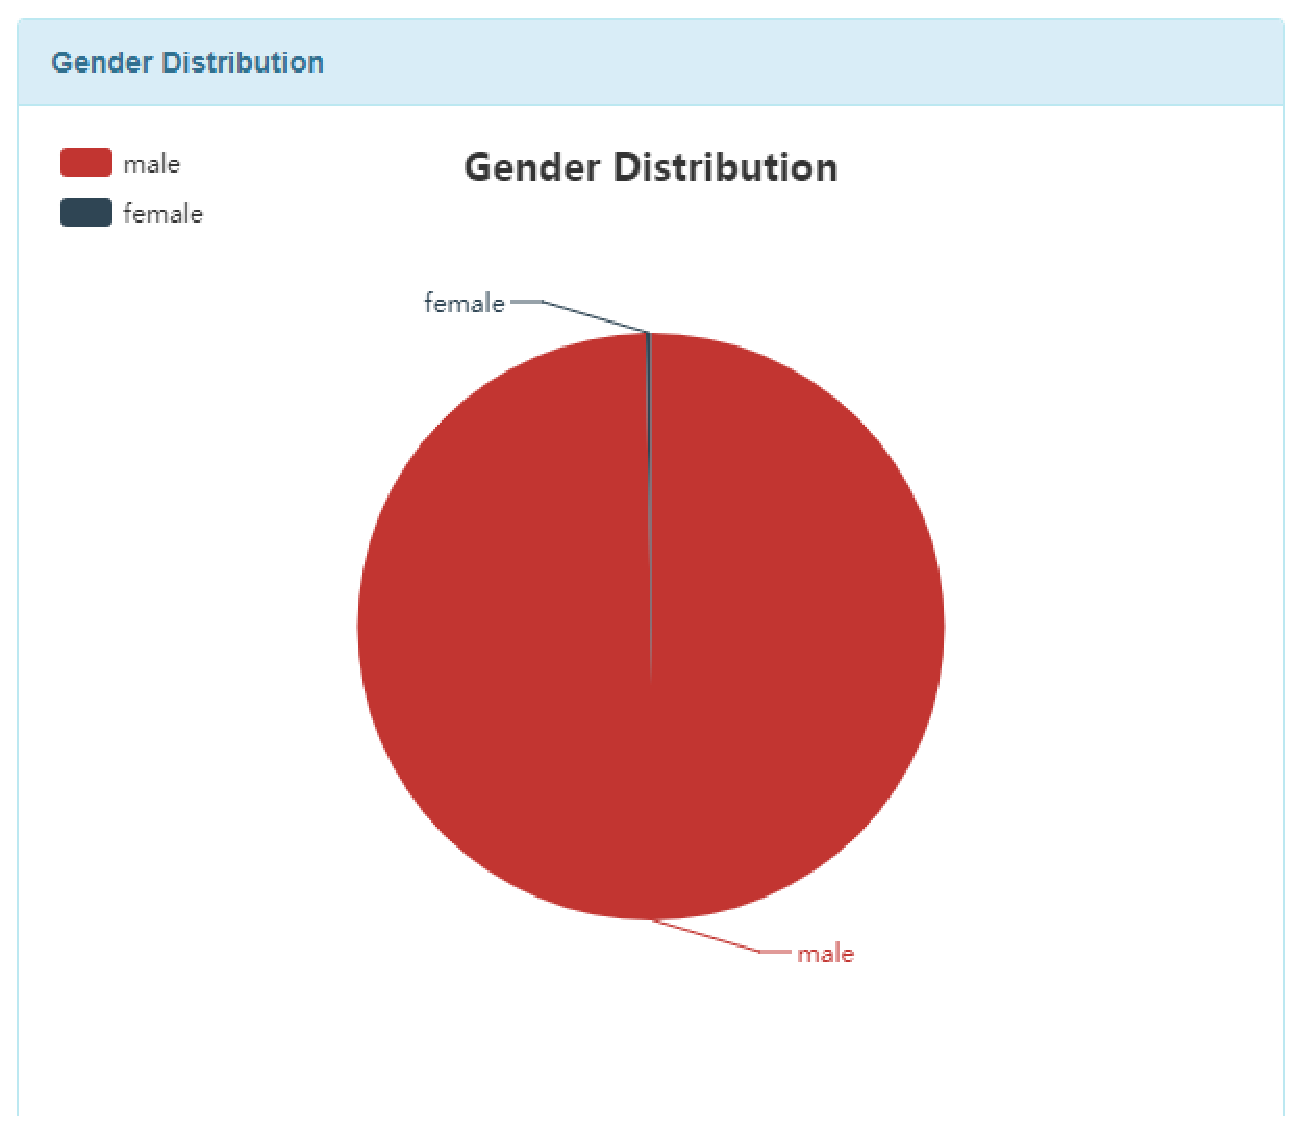
\includegraphics[width=0.23\textwidth]{IMAGE/group-images/31.eps}}
  \subfigure[]{
  \label{fig:subfig3:fig32}
      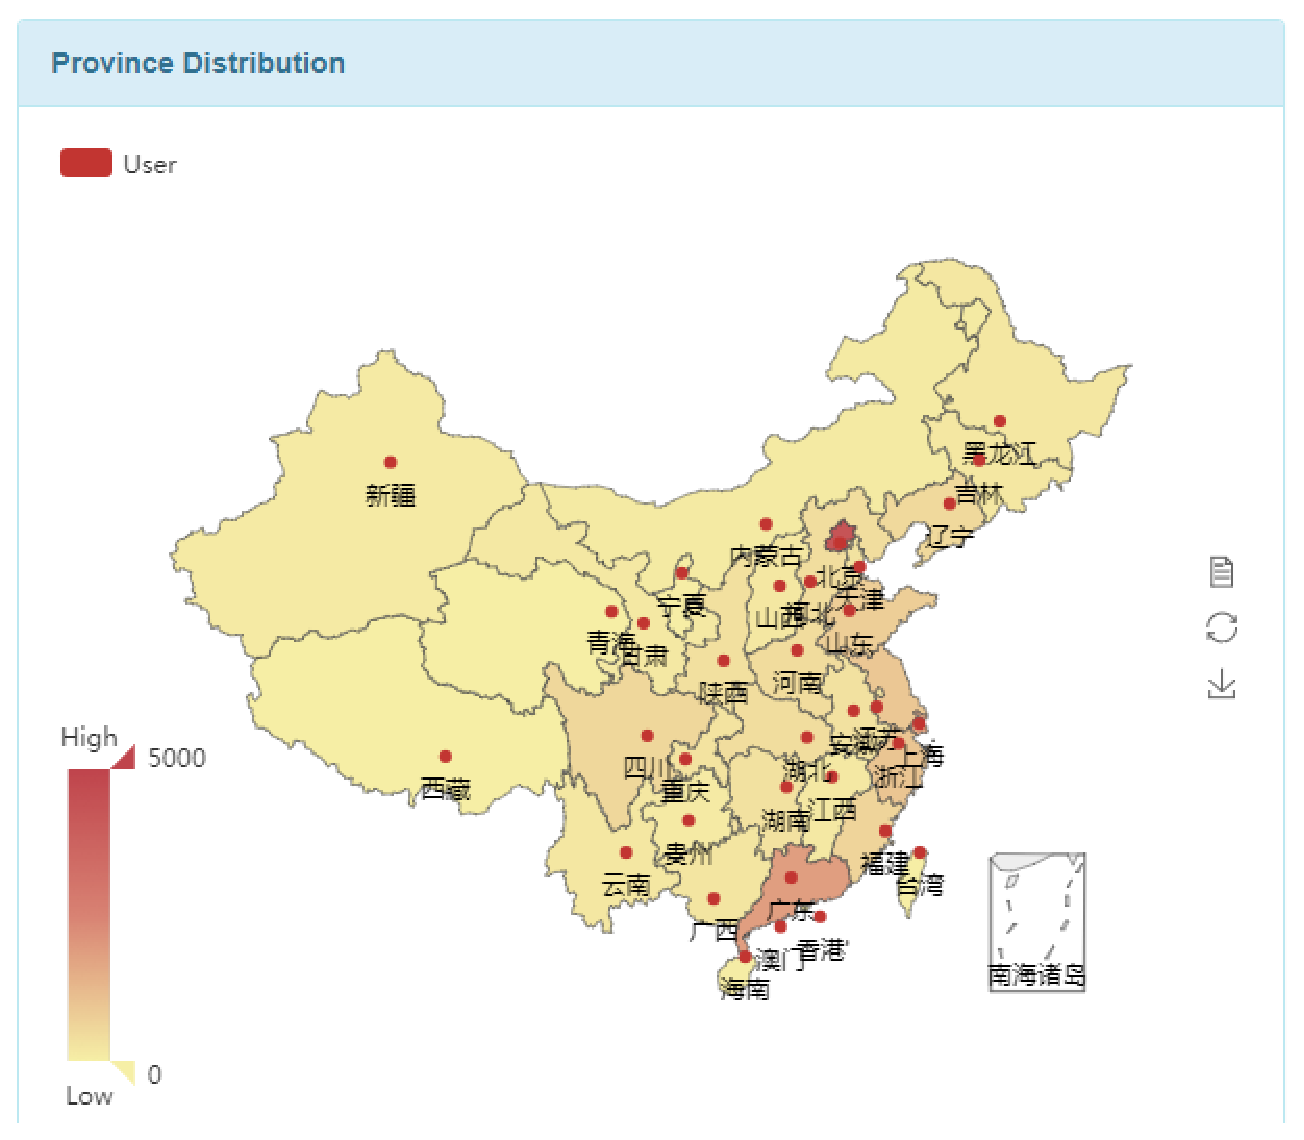
\includegraphics[width=0.23\textwidth]{IMAGE/group-images/32.eps}}
  \subfigure[]{
  \label{fig:subfig3:fig33}
      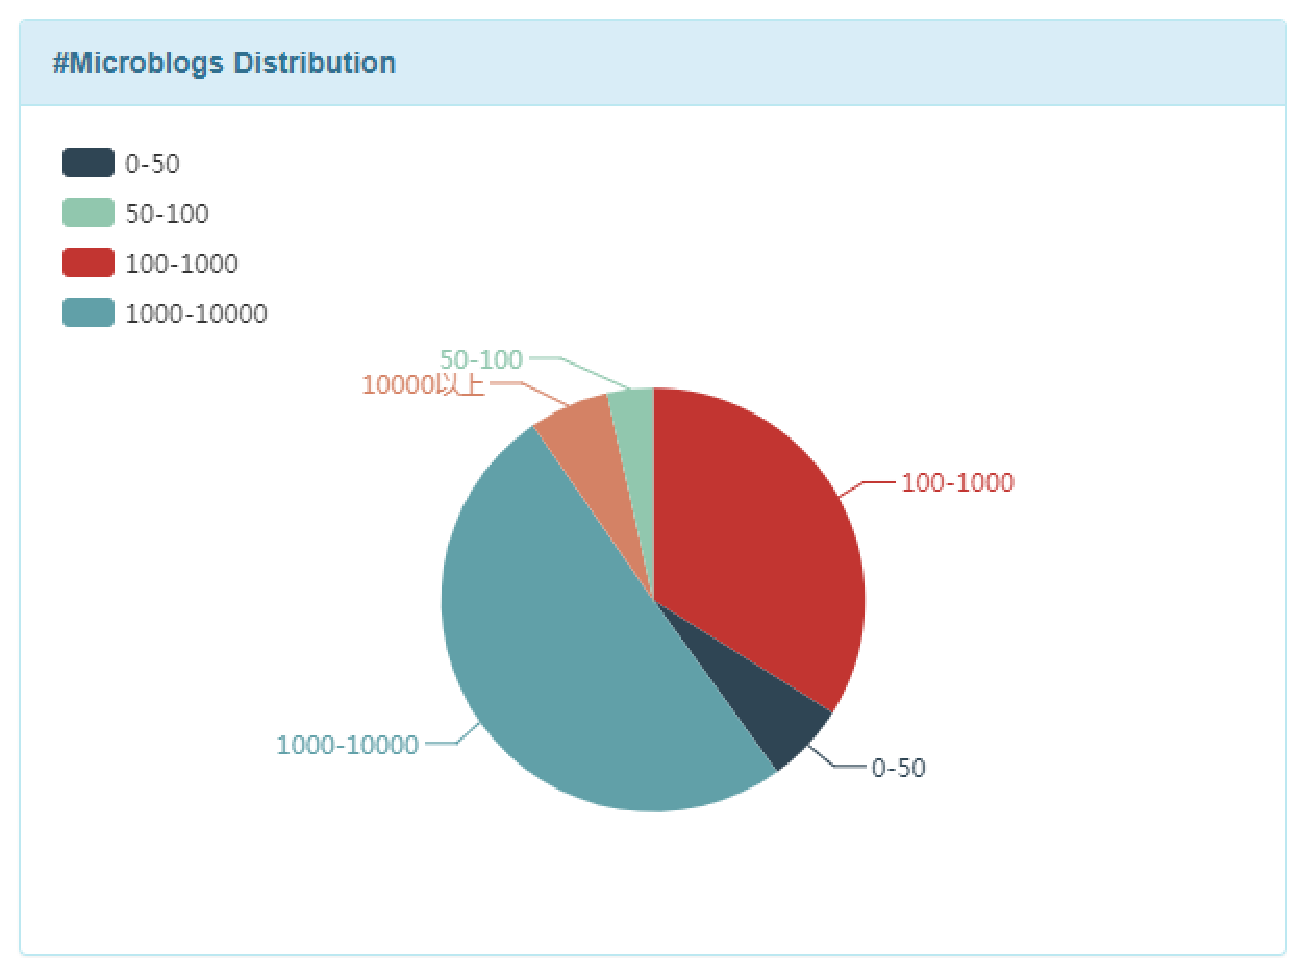
\includegraphics[width=0.23\textwidth]{IMAGE/group-images/33.eps}}
  \subfigure[]{
  \label{fig:subfig3:fig34}
      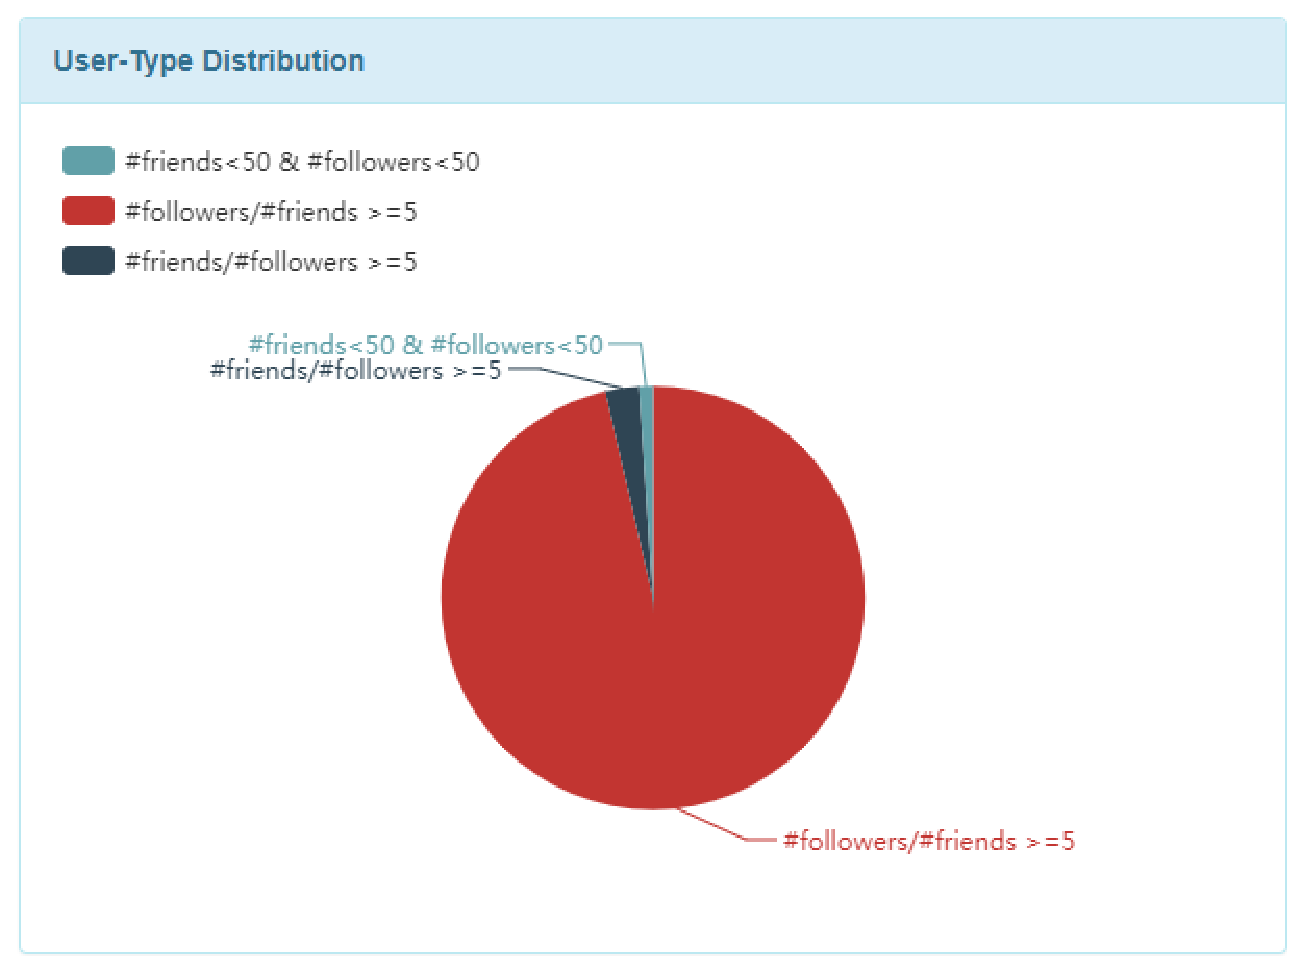
\includegraphics[width=0.23\textwidth]{IMAGE/group-images/34.eps}}
  \subfigure[]{
  \label{fig:subfig3:fig35}
      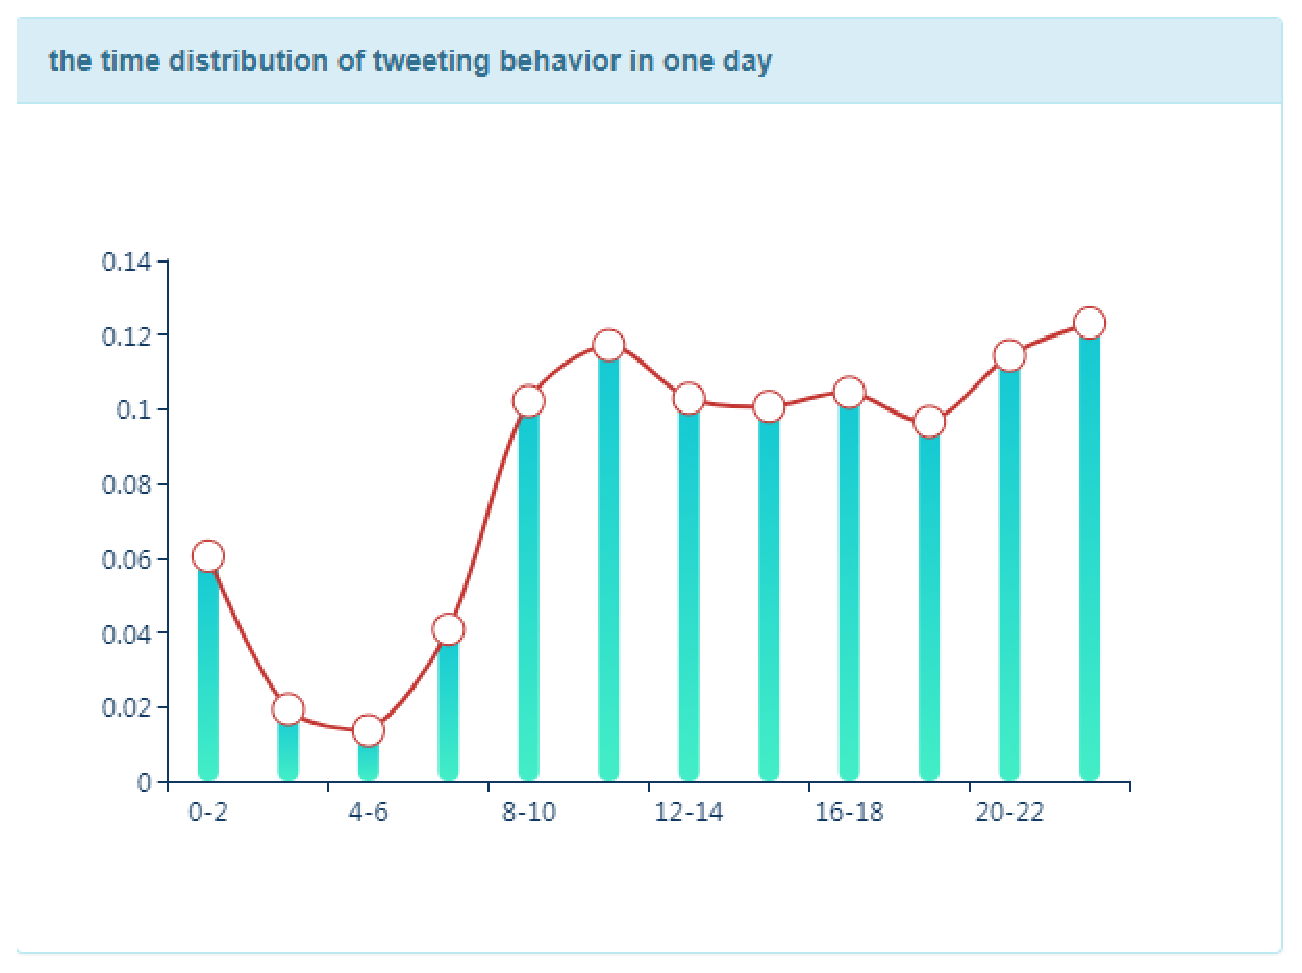
\includegraphics[width=0.23\textwidth]{IMAGE/group-images/35.eps}}
  \subfigure[]{
  \label{fig:subfig3:fig36}
      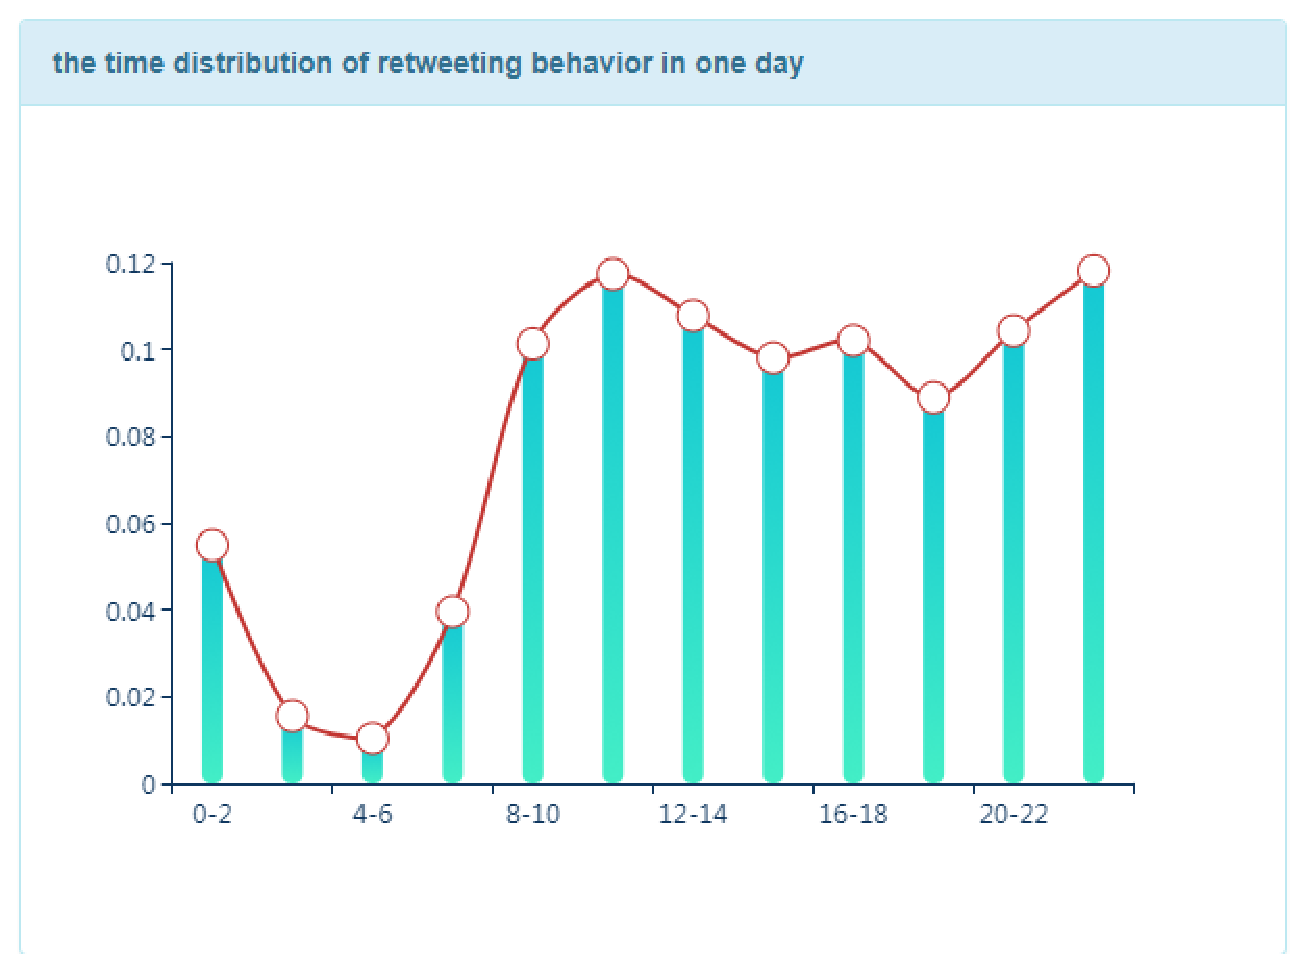
\includegraphics[width=0.23\textwidth]{IMAGE/group-images/36.eps}}
  \subfigure[]{
  \label{fig:subfig3:fig37}
      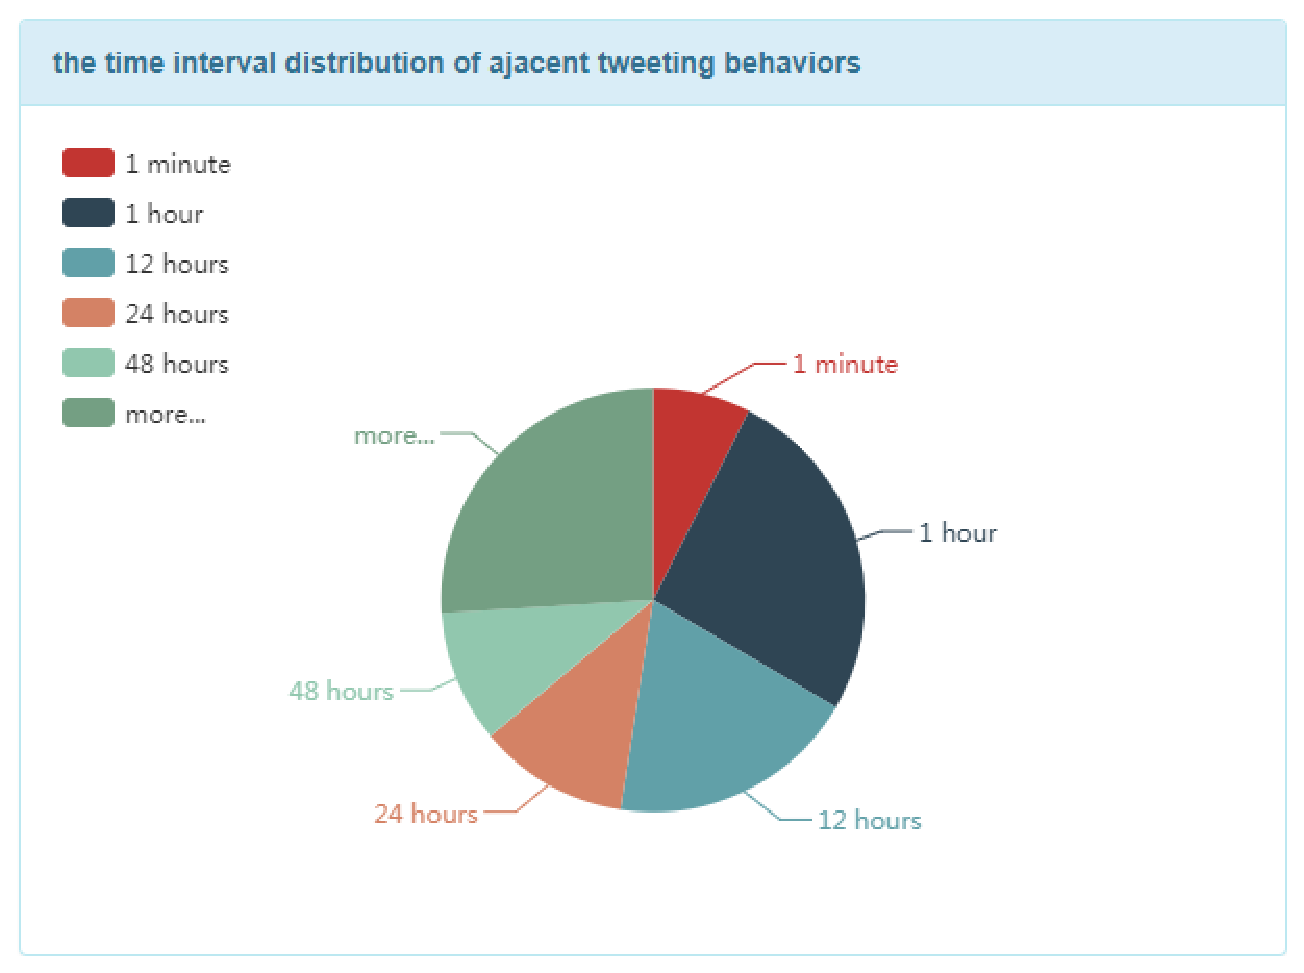
\includegraphics[width=0.23\textwidth]{IMAGE/group-images/37.eps}}
  \subfigure[]{
  \label{fig:subfig3:fig38}
      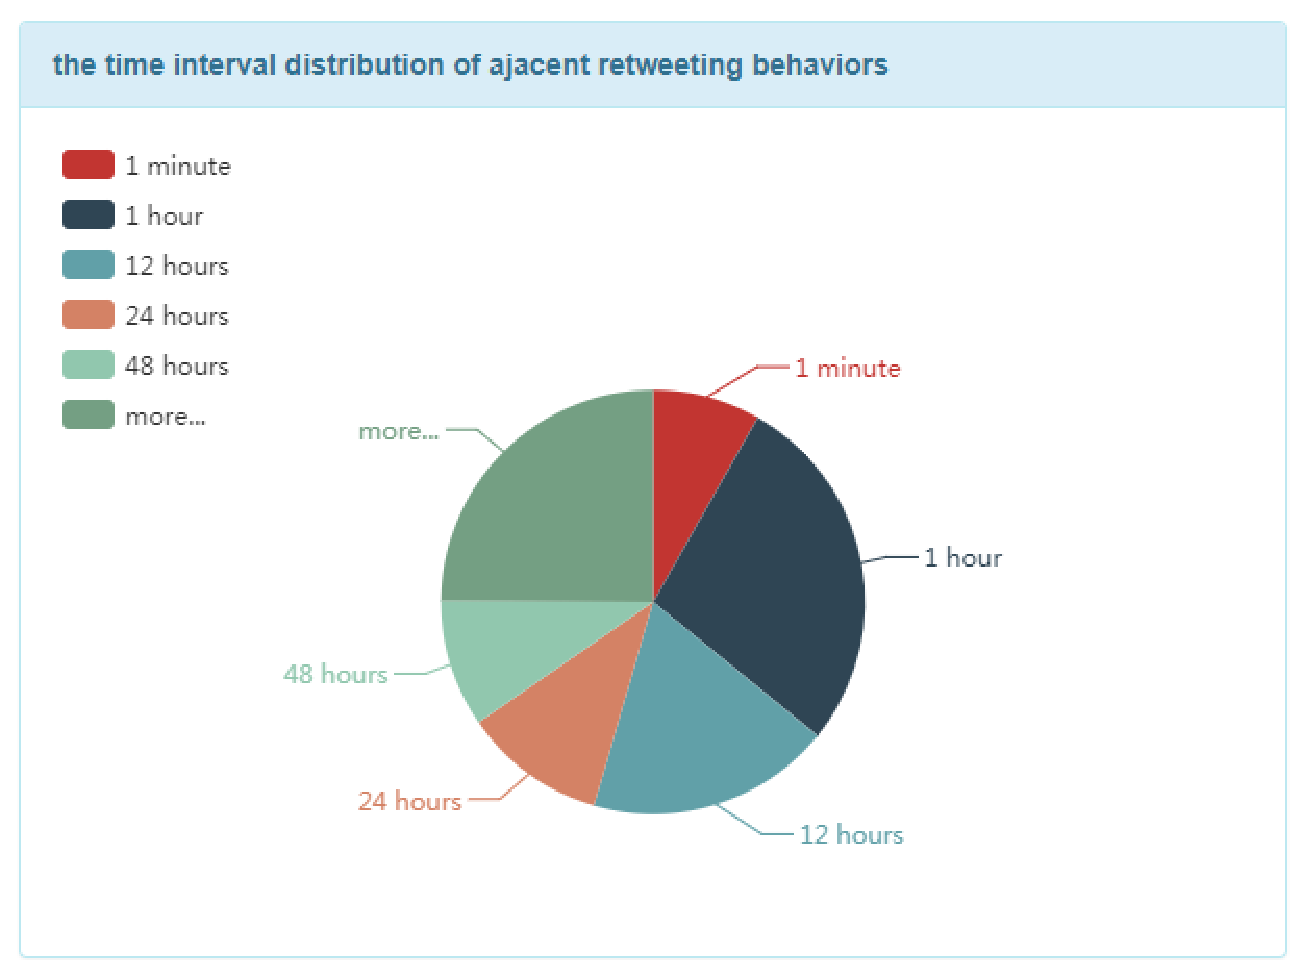
\includegraphics[width=0.23\textwidth]{IMAGE/group-images/38.eps}}
  \subfigure[]{
  \label{fig:subfig3:fig39}
      
\includegraphics[width=0.23\textwidth]{IMAGE/group-images/39.eps}}
  \caption{The Statistics of User Group Three}
  \label{fig:subfig3} %% label for entire figure
\end{figure*}


\begin{figure*}
  \centering
  \subfigure[]{
  \label{fig:subfig4:fig41}
      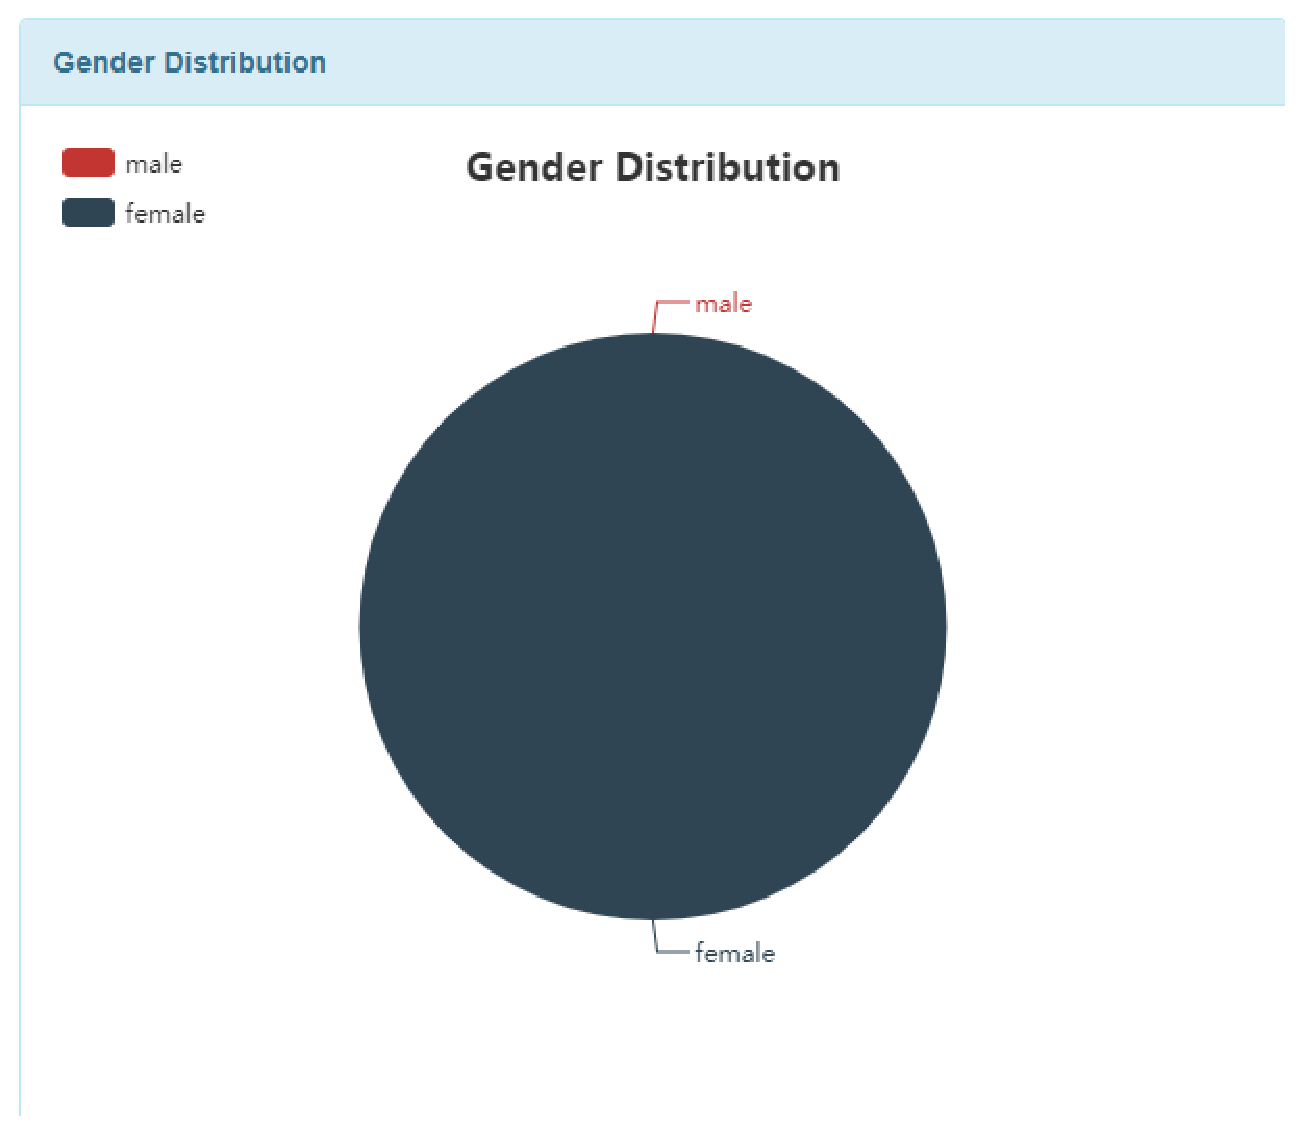
\includegraphics[width=0.23\textwidth]{IMAGE/group-images/41.eps}}
  \subfigure[]{
  \label{fig:subfig4:fig42}
      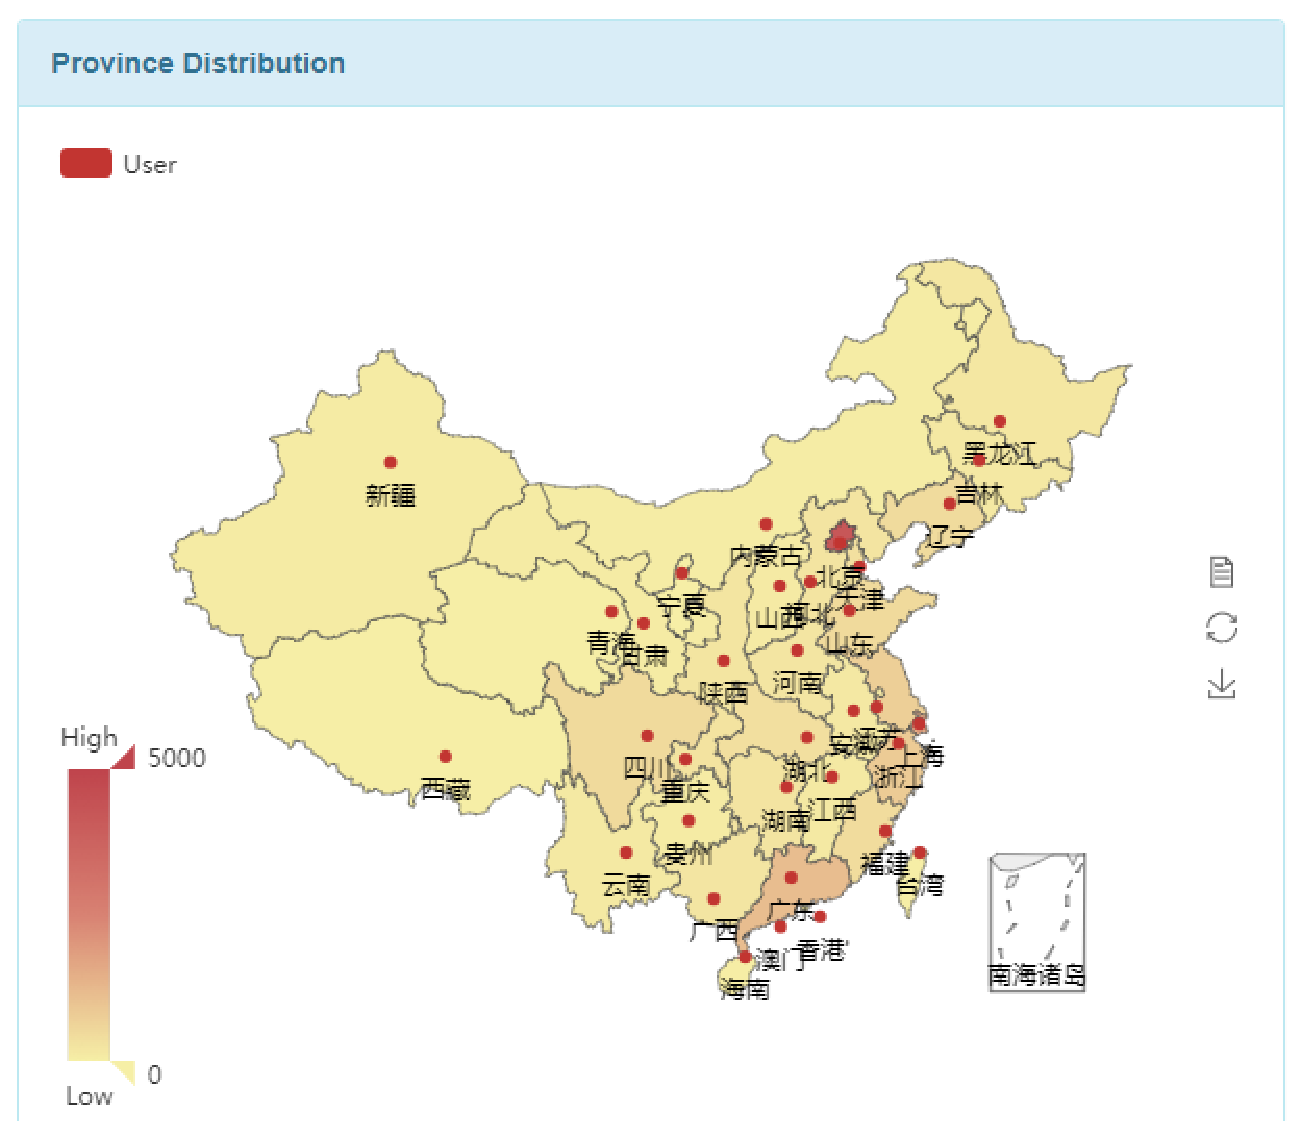
\includegraphics[width=0.23\textwidth]{IMAGE/group-images/42.eps}}
  \subfigure[]{
  \label{fig:subfig4:fig43}
      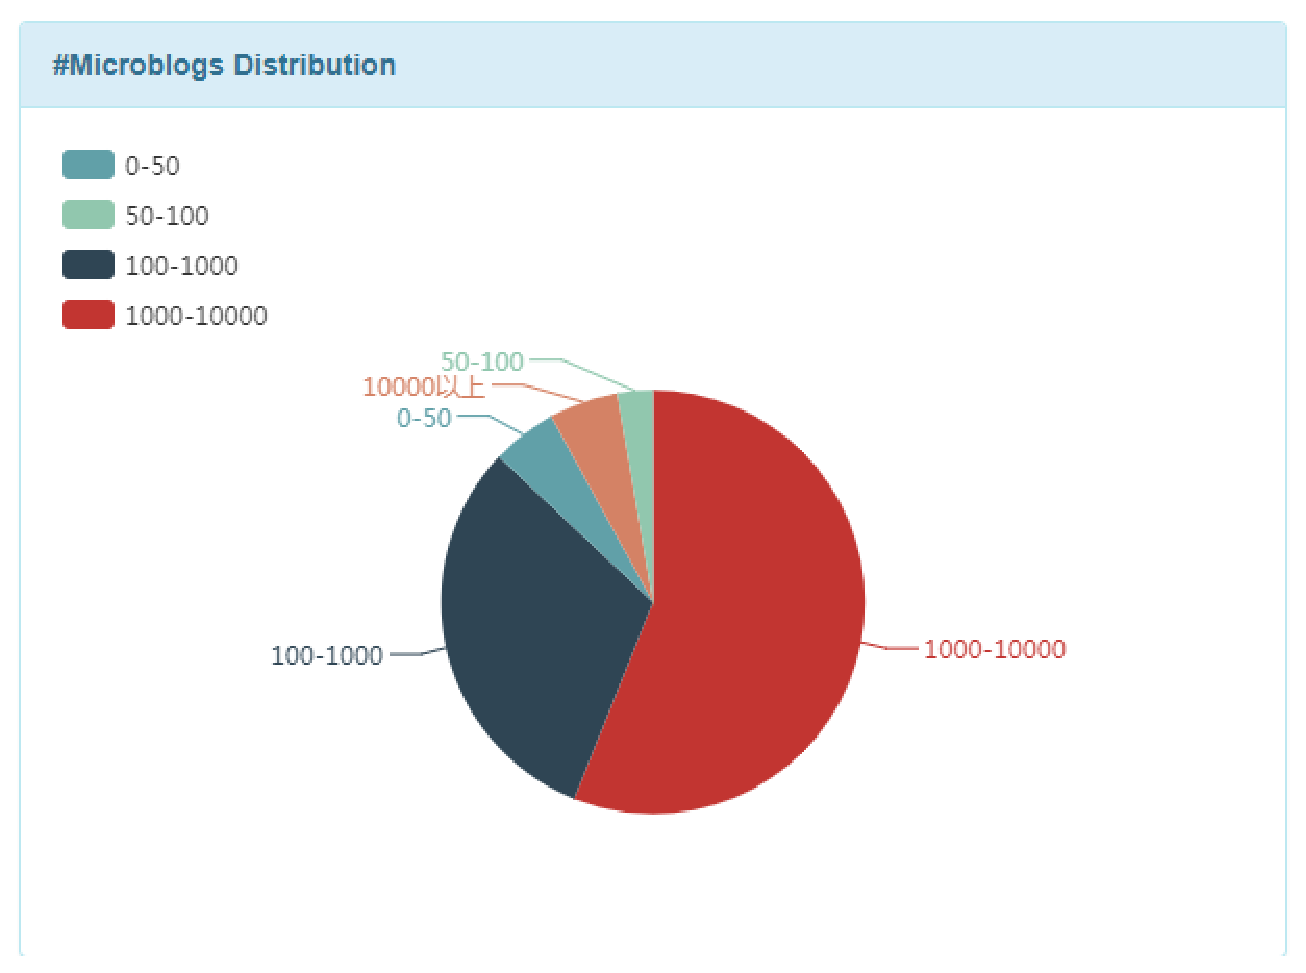
\includegraphics[width=0.23\textwidth]{IMAGE/group-images/43.eps}}
  \subfigure[]{
  \label{fig:subfig4:fig44}
      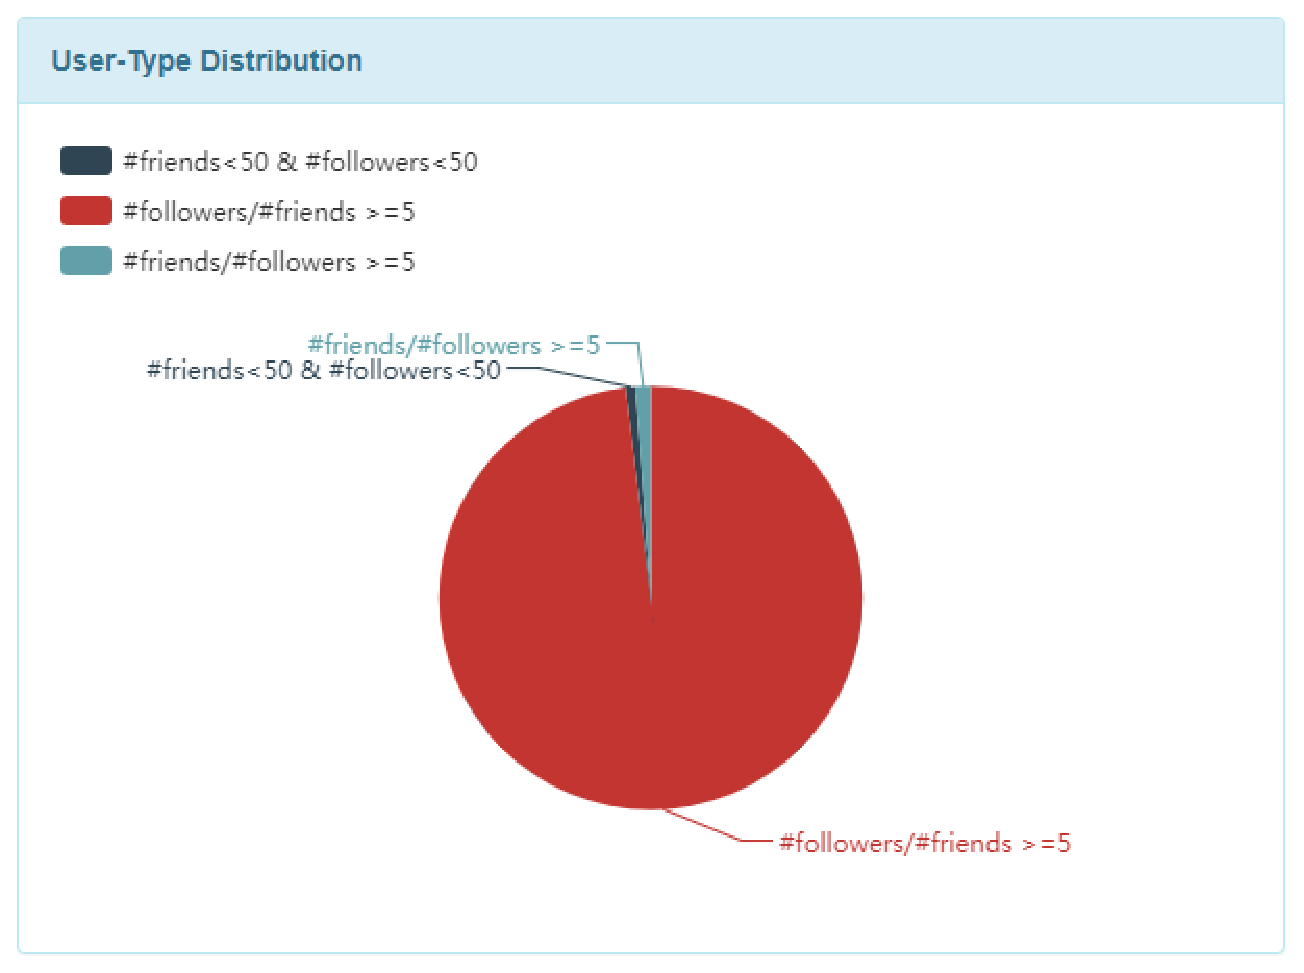
\includegraphics[width=0.23\textwidth]{IMAGE/group-images/44.eps}}
  \subfigure[]{
  \label{fig:subfig4:fig45}
      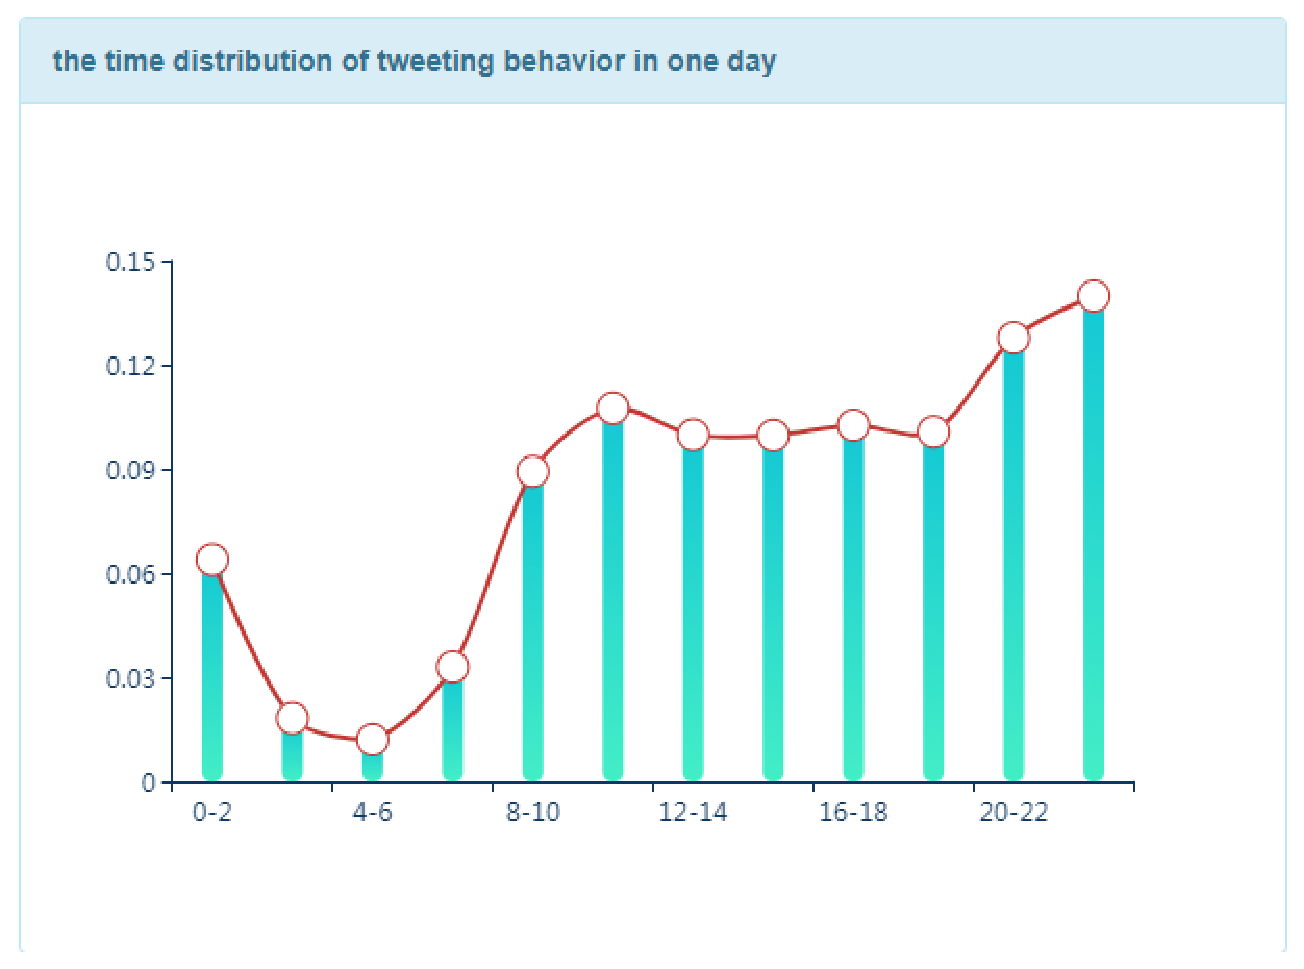
\includegraphics[width=0.23\textwidth]{IMAGE/group-images/45.eps}}
  \subfigure[]{
  \label{fig:subfig4:fig46}
      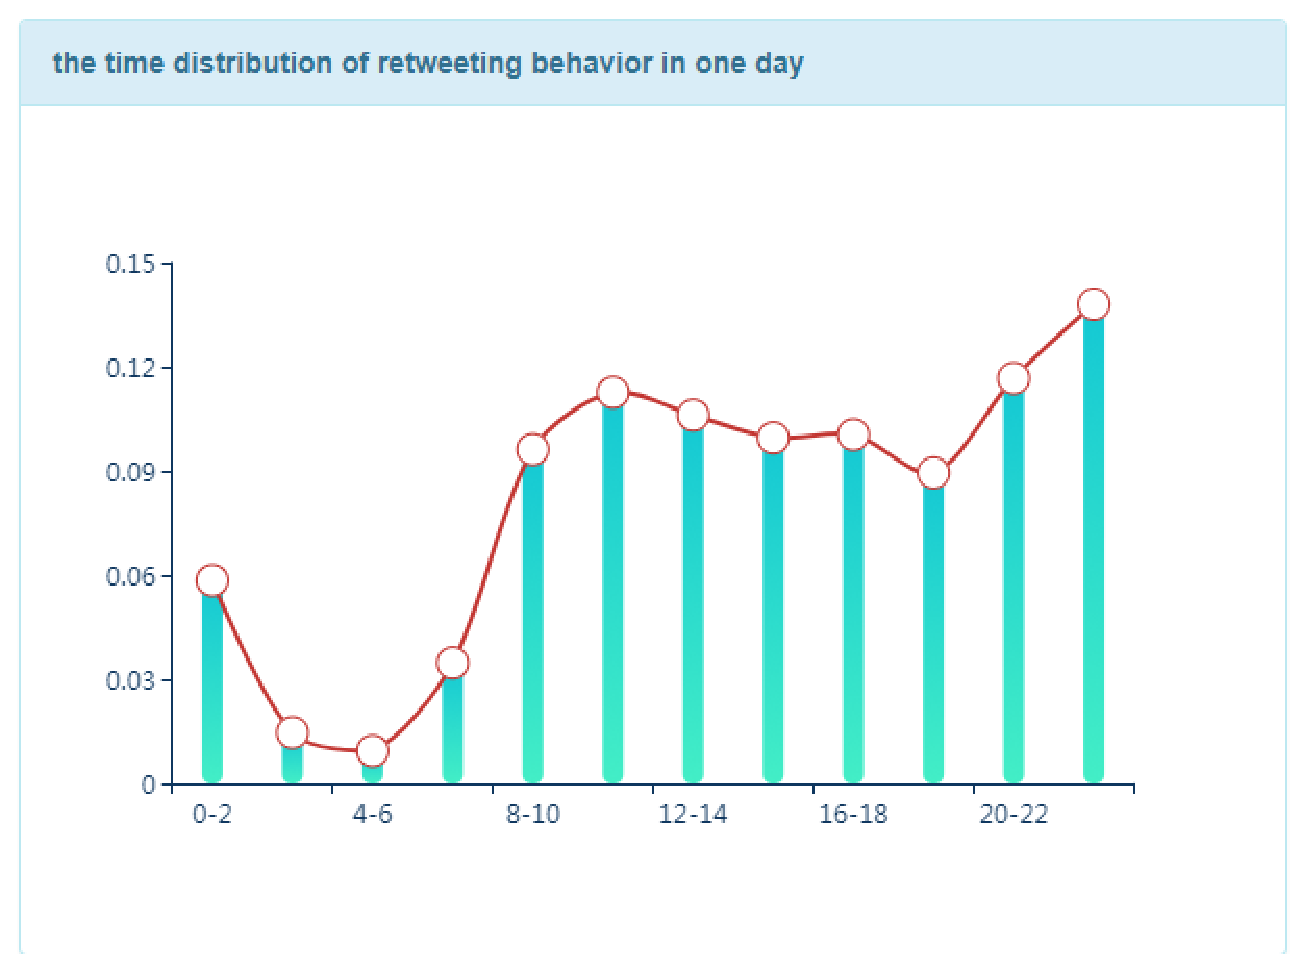
\includegraphics[width=0.23\textwidth]{IMAGE/group-images/46.eps}}
  \subfigure[]{
  \label{fig:subfig4:fig47}
      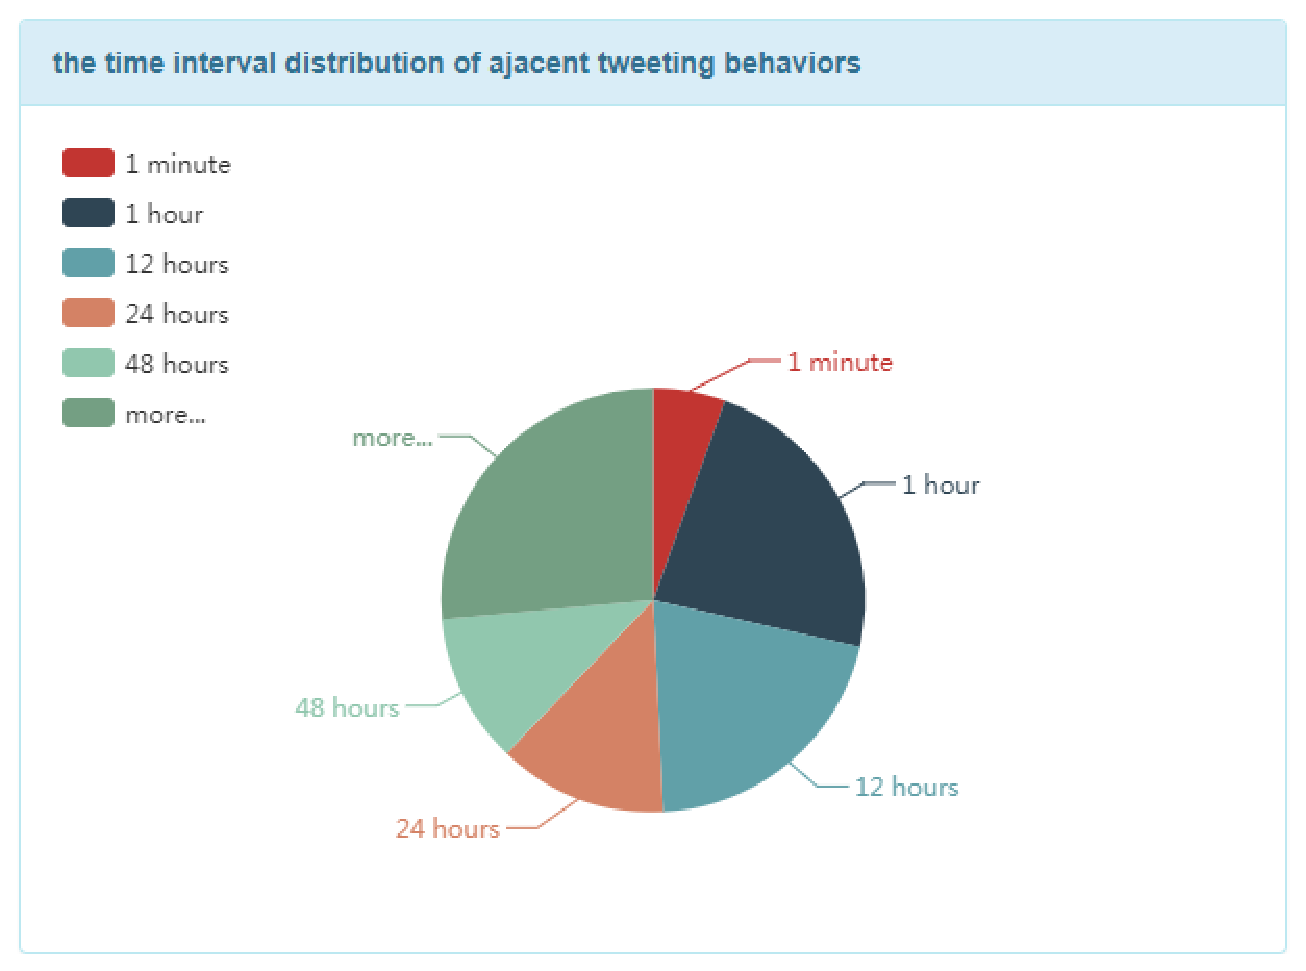
\includegraphics[width=0.23\textwidth]{IMAGE/group-images/47.eps}}
  \subfigure[]{
  \label{fig:subfig4:fig48}
      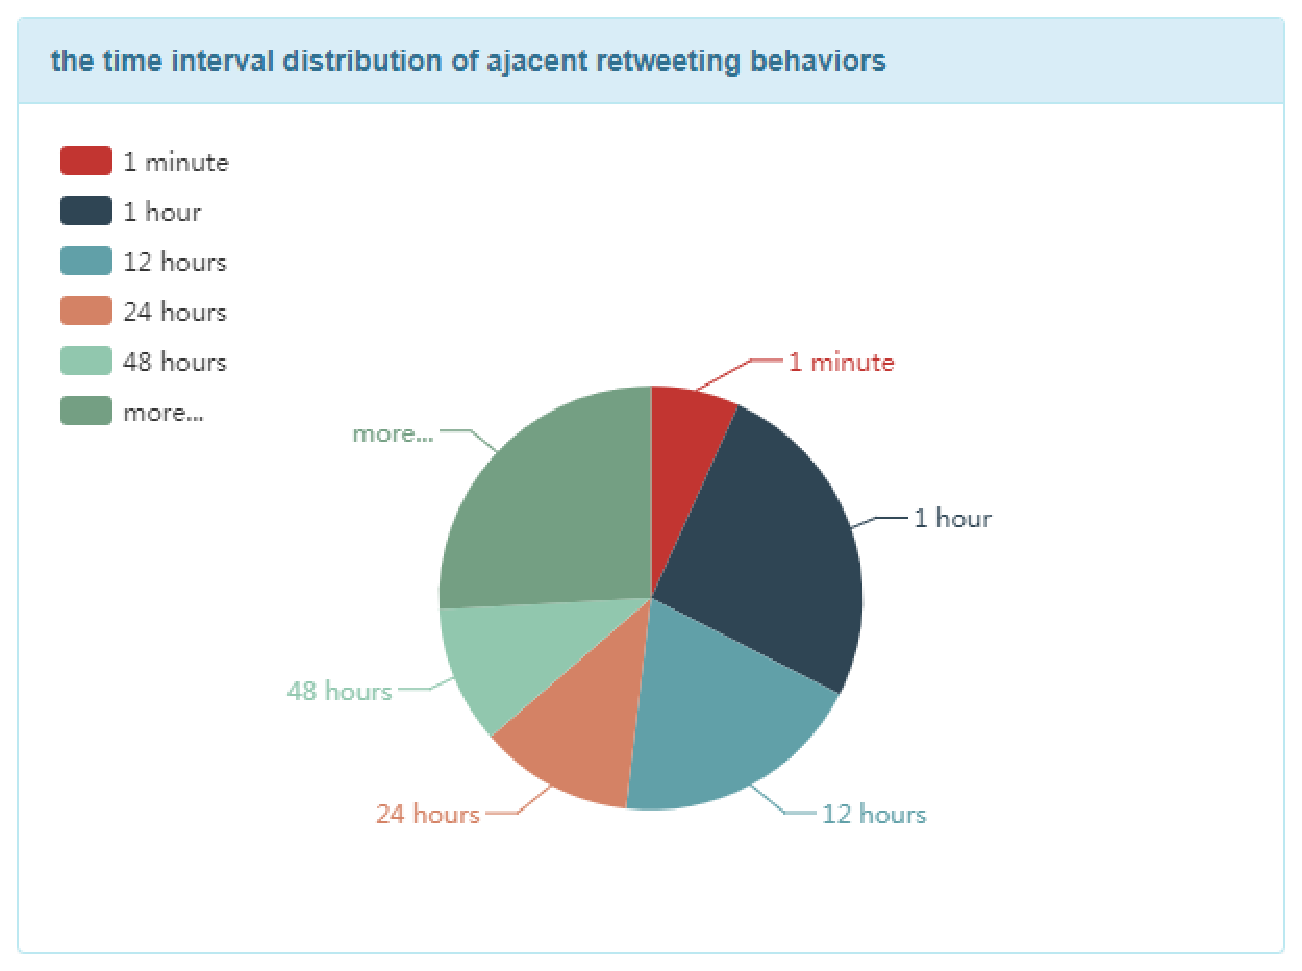
\includegraphics[width=0.23\textwidth]{IMAGE/group-images/48.eps}}
  \subfigure[]{
  \label{fig:subfig4:fig49}
      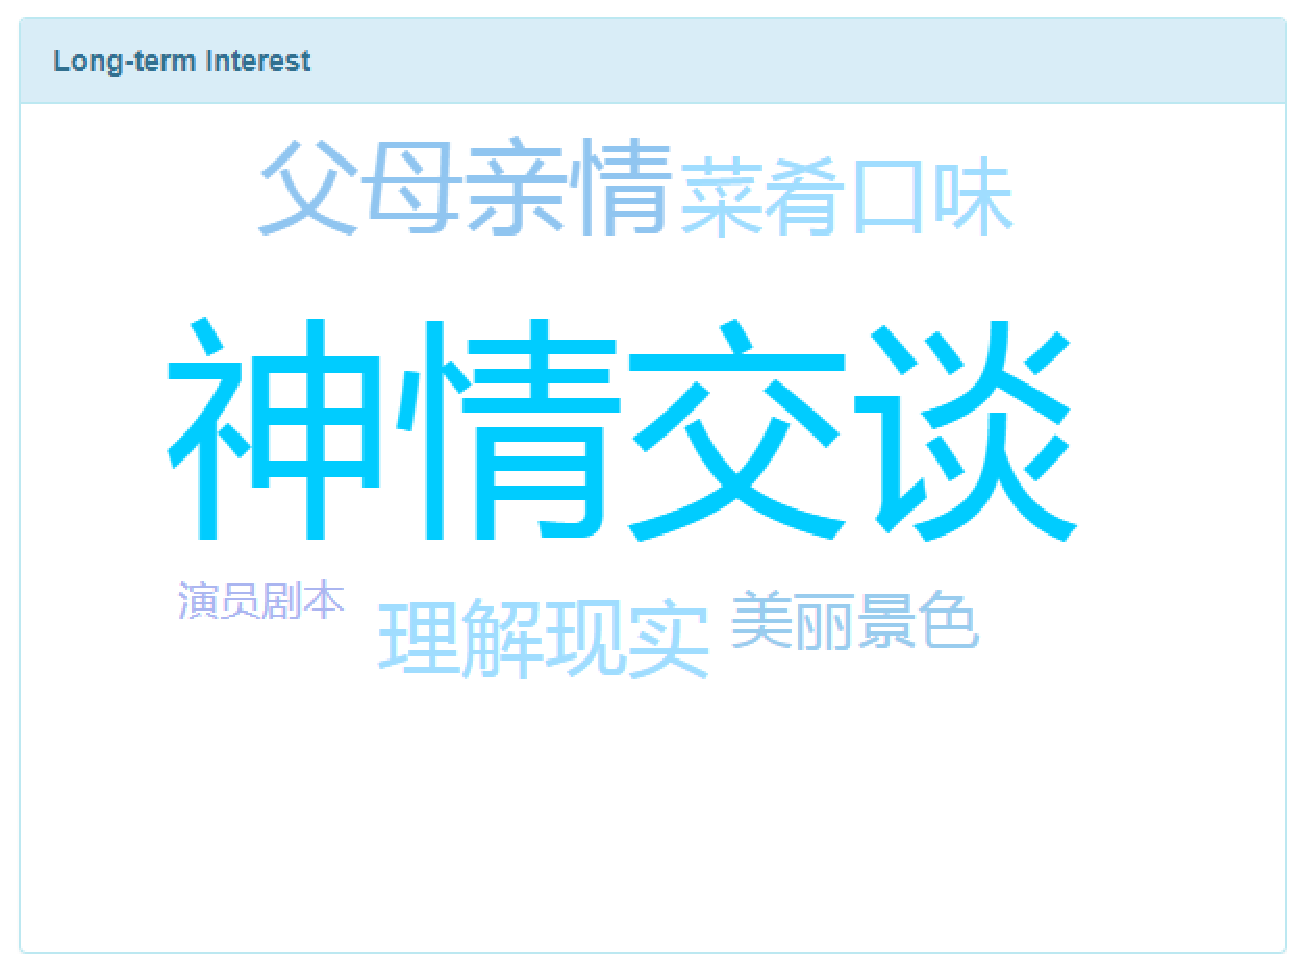
\includegraphics[width=0.23\textwidth]{IMAGE/group-images/49.eps}}
  \caption{The Statistics of User Group Four}
  \label{fig:subfig4} %% label for entire figure
\end{figure*}


\begin{table}[tb!]
\centering
\begin{small}
\caption{Variables}
\vspace{0.1cm}
\label{tbl:Variables1}
\begin{tabular}{lll}
\toprule
\multicolumn{1}{l}{\textbf{Variables}} & \multicolumn{1}{l}{\textbf{Illustration}}	& \multicolumn{1}{l}{\textbf{Section}} \\	\midrule \midrule
$M_b$             & a microblog     	  &2			\\	\midrule
$O$               & owner of a microblog           	  &2			\\	\midrule
$T$               & the generated time of a microblog	  &2			\\	\midrule
$M$               & the message context of a microblog	  &2			\\	\midrule
$flag$            & flag denoting $M_b$ is retweeted (1) or originally tweet (0) by O	  &2			\\	\midrule
$u$               & user $u$	  &2			\\	\midrule
$B_u$             & microblogs of user $u$	  &2			\\	\midrule
$R_u$             & followers of user $u$	  &2			\\	\midrule
$E_u$             & followees of user $u$	  &2			\\	\midrule
$\mathbb{U}$      & a set of users	  &2			\\	\midrule
$\mathbb{B}$      & a set of microblogs	  &2			\\	\midrule
$b$               & a microblog	  &2			\\	\midrule
$f$               & a follower	  &2			\\	\midrule
$G_u$				& gender of user $u$		        &3       		\\	\midrule
$P_u$				& province of user $u$				&3              \\	\midrule
                    & a ratio defined as the number     &         \\	
                    & of followers over that of         &3         \\		
\raisebox{1.5ex}{$R_{ee,u}$}  &followees,i.e.,$\frac{\#R_u}{\#E_u}$       &      \\  \midrule
$U_{t,u}$		    & user type (as illustrated in Table \ref{tbl:ucate}) &3        \\ \midrule	
$R_{oc,u}$          & ratio that is the number of retweeted microblogs over that of originally tweeted	  &3			\\	\midrule
$W_{r,u}$           & average number of retweeted microblogs per week	  &3			\\	\midrule
$W_{t,u}$           & average number of tweeted microblogs per week	  &3			\\	\midrule
$P_{rt,u}$          & normalized vector regarding the time distribution of a user��s retweeting  behavior	  &3			\\	\midrule
$P_{tt,u}$          & normalized vector regarding the time distribution of a user��s tweeting  behavior	  &3			\\	\midrule
$P_{rg,u}$          & normalized vector with respect to the gap distribution of a user��s retweeting behavior	  &3			\\	\midrule
$P_{tg,u}$          & normalized vector with respect to the gap distribution of a user��s tweeting behavior	  &3			\\	\midrule
$L$                 & A lexicon consists of a set of topics	  &3			\\	\midrule
$t$                 & A topic in $L$	  &3			\\	\midrule
$c$                 & A cell word in $L$	  &3			\\	\midrule
$P_u$               & The interest feature of a user $u$	  &3			\\	\midrule
$WS$                & a word set	  &3			\\	\midrule
$W_f$               & a metric TF-IDF weight	  &3			\\	\midrule
$b_i$               & the occurrences of word $w_i$ in microblog $b$	  &3			\\	\midrule
$|D_i|$             & the number of microblogs which contains word $w_i$	  &3			\\	\midrule
$|D|$               & the number of all microblogs	  &3			\\	\midrule
$N_t$               & the number of words in topic $t$	  &3			\\	\midrule
$W_w$               & A metric Twitter-LDA weight	  &3			\\ \bottomrule
\end{tabular}
\end{small}
\end{table}

\begin{table}[tb!]
\centering
\begin{small}
\caption{Variables}
\vspace{0.1cm}
\label{tbl:Variables2}
\begin{tabular}{lll}
\toprule
\multicolumn{1}{l}{\textbf{Variables}} & \multicolumn{1}{l}{\textbf{Illustration}}	& \multicolumn{1}{l}{\textbf{Section}} \\	\midrule \midrule
$\alpha$            & a parameter set flexible priorities between TF-IDF and Twitter-LDA	  &3			\\	\midrule
$t_k$               & a topic in $L$	  &3			\\	\midrule
$b_m$               & a microblog of user $u$	  &3			\\	\midrule
$B_s(u)$            & microblogs of user $u$	  &3			\\	\midrule
$s_k$               & overall similarity of user $u$ over topic $t_k$	  &3			\\	\midrule

$Y'$,$Z'$           & numerical vectors	  &4			\\	\midrule
$Y''$,$Z''$          & categorical vectors	  &4			\\	\midrule
$Y^{\ast}$,$Z^{\ast}$     & vectors where each dimension is a normalized vector per se	  &4			\\	\midrule
$d_i(u)$            & the average distance to all the other users in the same cluster	  &4			\\	\midrule
$d_o(u)$            & the minimum of the distances between $u$ and other clusters	  &4			\\	\midrule
$v(u)$              & The Silhouette coefficient value	  &4			\\	\midrule

$E$                 & An item $E$ involves a microblog $b$ and a user $f$ such that $f\ \in R_{b.O}$	  &5			\\	\midrule
$C_h$               & the correlation metric $C_h$ of $b$ and event	  &5			\\	\midrule
$W_s$               & $u$'s short-term interest	  &5			\\ \bottomrule
\end{tabular}
\end{small}
\end{table}


\begin{table}[tb!]
\centering
\begin{small}
\caption{Variables}
\vspace{0.1cm}
\label{tbl:Variables2}
\begin{tabular}{ll|ll}
\toprule
\multicolumn{1}{l}{\textbf{Variables}} & \multicolumn{1}{l}{\textbf{Illustration}}
& \multicolumn{1}{l}{\textbf{Variables}} & \multicolumn{1}{l}{\textbf{Illustration}} \\	\midrule \midrule
$L$                 & A lexicon consists of a set of topics	
&$t$                 & A topic in $L$	 			\\	\midrule
$c$                 & A cell word in $L$	
&$P_u$               & The interest feature of a user $u$	 			\\	\midrule
$WS$                & a word set	 			
&$W_f$               & a metric TF-IDF weight				\\	\midrule
$b_i$               & the occurrences of word $w_i$ in microblog $b$	
&$|D_i|$             & the number of microblogs which contains word $w_i$			\\	\midrule
$|D|$               & the number of all microblogs
&$N_t$               & the number of words in topic $t$				\\	\midrule
$W_w$               & A metric Twitter-LDA weight
&$\alpha$            & a parameter set flexible priorities between TF-IDF and Twitter-LDA			\\	\midrule
$t_k$               & a topic in $L$	
&$b_m$               & a microblog of user $u$			\\	\midrule
$B_s(u)$            & microblogs of user $u$	
&$s_k$               & overall similarity of user $u$ over topic $t_k$			\\	\bottomrule
\end{tabular}
\end{small}
\end{table}




\begin{table}[]
\centering
\caption{My caption}
\label{my-label}
\begin{tabular}{|l|l|l|l|}
\hline
\alpha & accuracy & precision & recall &  \\ \hline
0	&0.488500	&0.636667	&0.560833     \\ \hline
0.1	&0.479167	&0.633333	&0.557500     \\ \hline
0.2	&0.481333	&0.636667	&0.564167     \\ \hline
0.3	&0.506500	&0.663333	&0.588333     \\ \hline
0.4	&0.497167	&0.660000	&0.587500     \\ \hline
0.5	&0.497583	&0.666667	&0.600833     \\ \hline
0.6	&0.524417	&0.693333	&0.622500     \\ \hline
0.7	&0.576583	&0.720000	&0.649167     \\ \hline
0.8	&0.502250	&0.650000	&0.590833     \\ \hline
0.9	&0.450583	&0.596667	&0.550833     \\ \hline
1	&0.396417	&0.536667	&0.501667     \\ \hline
\end{tabular}
\end{table}

















